\documentclass{article}
\usepackage{graphicx} % Required for inserting images
\usepackage[margin=1in]{geometry}
\usepackage[backend=biber,style=authoryear,
sorting=nyt]{biblatex}


\bibliography{refs}

\title{Using Messy Text In  Future LLM Annotations.\footnote{This research was supported by NSF award OAC-2311142 and 
used Delta at NCSA / University of Illinois through allocation CIS220162 from the Advanced Cyberinfrastructure Coordination Ecosystem: Services \& Support (ACCESS) program, which is supported by NSF awards 2138259, 2138286, 2138307, 2137603, and 2138296. Any opinions, findings, and conclusions or recommendations expressed
in this material are those of the author(s) and do not necessarily
reflect the views of the National Science Foundation,  NCSA, or the
affiliated university resource providers.}}

\author{Patrick Brandt \\ School of Economic, Political and \\ Policy Sciences \\ University of Texas, Dallas\\ \email{pbrandt@utdallas.edu}
\and Shreyas Meher \\ Erasmus School of Social and\\ Behavioural Sciences\\ Erasmus University \\
%\\ Rotterdam, Netherlands \\
\email{meher@essb.eur.nl}
\and Paula Cuellar-Cuellar \\ Bass School of Arts, \\ Humanities and Technology \\ \email{email}  \\ University of Texas, Dallas\\
\and Xingyaun Zhao \\ School of Economic, Political and \\ Policy Sciences \\ University of Texas, Dallas\\ \email{email}}
\date{\today}

\begin{document}


\maketitle
\begin{abstract}
% Some abstract here    

% TWO BIG THINGS:

% - Use the codebook to focus attention of the LLM: all you need is codebook attention
% - Use the turn-by-turn results to show where the errors are and document the cost of additional turns and annotations (so make explicit the human and machine trade).

When working with real-world text, researchers often inherit corpora and annotations with costly human judgments but were not collected, organized, or annotated for modern text-as-data workflows. This is especially common in social science domains where web-scraped documents are noisy, incomplete, or misaligned with the unit of analysis.
We propose \emph{codebook attention}: a codebook-guided turn-by-turn extractive summarization pipeline that reuses valuable annotations without requiring full re-annotation. For each victim in a corpus of disappearance reports from Mexico, the model processes documents sequentially, extracts verbatim evidence spans for each codebook category, and updates a running structured summary to produce a clean and evidence-traceable document-level representation. Using the codebook as the task schema focuses model attention on the fields that matter for downstream classification and reconnects prior human annotations to contemporary language model workflows. We evaluate the resulting summaries by classifying and comparing the predicted labels with human annotations across multiple open-source models. %Because the pipeline records turn-by-turn outputs, it also identifies where errors enter the workflow and documents the marginal gains and costs of additional turns and annotations, making the human and machine trade explicit. Preliminary 
Results suggest that hours of computation can approximate weeks of human coding effort while producing evidence-traceable summaries suitable for downstream human rights and event data research.
\end{abstract}

\newpage

\section{Introduction}\label{introduction}

% Needs an intro here to set up the problem: how do we use / re-use annotations of texts and corpora that were not originally gathered, organized or even annotated to the standards of modern LLM methodology standards?

Many valuable text data and annotations were created before the standards and data structures now expected in LLM based research. These materials preserve costly human judgment and domain knowledge, yet they were often not gathered, organized, or annotated in ways that make them directly usable for contemporary computational workflows. This creates a central research problem: how can researchers use or reuse legacy texts and annotations without losing their original knowledge while making them usable for modern LLM based analysis.

Our goal is to reuse the prior data collection and annotations to create a balanced and clean corpus. Addressing downstream tasks using real-world data, researchers often must work with a messy and noisy texts. These texts can contain irrelevant formatting and information resulting from poor web scraping, connection errors, or faulty parsing, such as navigation menus, error pages, cookie consent notices, and social media sharing buttons interspersed with article content. What might be worse is that, these texts might contain seemingly related but essentially unrelated information as distractions, originating from suggested articles or user comments on the article page. Additionally, these texts might not be organized or structured in a way that is ready for processing by modern text-as-data methods.

\emph{Humans can easily filter and extract around this noise and may have already done so to produce annotations}.  But to extend this with the latest LLMs one needs to a) clean the texts (explicitly) and b) reconnect the human annotations to the modern needs to LLMs (e.g., span annotations rather than just words or linkages to actual images in a larger document) (\cite{olsen-etal-2024-socio}). 

Solving these problems allows researchers to work with and re-use texts for their research but that are currently messy and not well-structured. Our application is a corpus on disappearance cases that is valuable and significant for human rights' research as well as serving training for the classification and prediction of future abduction cases. We propose a multi-turn extractive summarization method that sequentially processes the original messy and disorganized documents for each unit of analysis (victim).  This is done with a conversation state that iteratively updates the running summary with exact text spans from new documents, generating a summary by item for each victim, comprised of sentences extracted from the report that are directly relevant to the item.

%\subsection{Contributions}\label{contributions}

Researchers may encounter a mismatch between collected data and the
target unit of analysis. Since this work addresses this problem through
LLM-based alignment, our work contributes a generalizable approach so
that other source-task or annotation-task discrepancy can be resolved
without re-collection using human coders that is expensive,
time-consuming and vulnerable to knowledge loss. Researchers may also
encounter the need to perform document level de-duplication and
information extraction across sources reporting the same events. Our
work addresses the case where multiple reports must be aggregated into
unified data fields, it contributes an extractive AI approach so that
redundant information across documents can be consolidated and traced
back to the original sources without manual effort.

This work also demonstrates a better way of using LLMs to assist social
science research. LLMs are powerful tools but are also
vulnerable to hallucination and other biases if not used carefully. We provided a framework that is more robust to hallucination and other biases by using a multi-turn stateful workflow framework that maintains
context across operations. The more important part is that our framework
allows tracking the source and evidence of the information extracted
from the text, which bridges the gap between the annotations and the
lost knowledge of the original coders.

\medskip

Contribution to downstream tasks: 

- Fine-tuning: We can use the
summaries to fine-tune the models to improve the performance of the
models. (Shreyas)

\medskip

Human rights research relies on vast bodies of documentation—including court records, testimonies, NGO reports, forensic evidence, media archives, and government materials—that often exceed the capacity of traditional qualitative methods. Cleaned and well-organized corpora transform these fragmented materials into searchable datasets, enabling researchers and organizations to navigate complex documentation more efficiently and connect sources that would otherwise remain dispersed across institutions, languages, and formats.

Once documentation is systematically organized, computational tools such as large language models (LLMs) can significantly expand analytical capacity. They assist with tasks such as entity extraction, document classification, timeline reconstruction, and cross-referencing events across large collections of records. Rather than replacing expert judgment, these tools reduce the time required for large-scale document review and allow human rights investigators to concentrate on verification, contextual interpretation, and legal analysis.

Standardized documentation systems also strengthen methodological consistency across research projects. Human rights investigations are often collaborative and extend across long periods of time. Using common variables, metadata structures, and coding protocols allows multiple researchers and institutions to contribute to a shared body of evidence. This facilitates cumulative research, improves transparency, and ensures that documentation collected today remains usable for future investigations, historical analysis, and accountability processes.

These systems are particularly important for local NGOs and independent human rights researchers, who frequently operate with limited funding, infrastructure, and personnel. Grassroots organizations are often the primary collectors of crucial evidence—such as testimonies, photographs, and local reports of abuses—but may lack the capacity to process large archives of material. Clear and standardized datasets make it easier for these organizations to integrate the information they gather into broader evidentiary frameworks without requiring extensive technical resources.

Accessible and well-structured documentation systems also help empower victims and affected communities. When information is organized through clear categories—such as dates, locations, types of violations, and responsible actors—it becomes easier to understand what kinds of information are most relevant to collect and preserve. Because many victims lack the economic resources, technical skills, or literacy needed to manage complex documentation systems, accessible formats lower these barriers and allow communities to store, access, and interpret the evidence they produce. In this way, structured corpora not only strengthen research capacity but also support victims’ participation in processes of truth, historical reconstruction, and justice.


\section{Related Work}\label{related-work}

We review and consider three approaches for aligning and re-using our prior texts and their annotations.  These are detailed below as \emph{non-LLM methods}, and \emph{LLM-methods} both of which are mainly extractive approaches that would either use human or text-as-data methods.  The final approach we advocate and develop is a hybrid approach that uses both generative and extractive LLM methods, which we call \emph{extraction and summarization} (see \cite{Brandt_etal2025} for a discussion of these distinctions). 

\subsection{Non-LLM Methods for Messy
Text}\label{non-llm-methods-for-messy-text}

Producing a clean, structured dataset from noisy web-scraped text while preserving traceable connections to the original source material is a problem that has a lot of needs to be addressed before the invention of LLM models.

Note that we cannot use something like this because we only have a messy version of the text that the human coder saw initially.  So we do not know the visual layout of the original documents or what was lost in archiving the text to document and justify the annotations for each victim.

Typically, researchers uses rule-based preprocessing, manual data cleaning, or a combination of both to clean and organize raw text data (\cite{Bohannon_etal2007}, \cite{OpenRefine2025}).

Rule-based methods represent the most common preprocessing approach for noisy text. These methods apply fixed text operations such as regular expression matching, HTML tag stripping, stopword removal, and pattern-based filtering to remove structural artifacts from scraped documents. Although they are computationally inexpensive and easy to implement, their effectiveness is constrained by the heterogeneity of web content. Because each source website uses a different page layout, a rule set calibrated to one domain does not generalize reliably to others, and there is no guarantee that the same pattern will identify the same type of noise across sources. More critically, rule-based approaches is hard to understand the nuances of the text and cannot handle semantically related but contextually irrelevant content (\cite{Rahm2011}, \cite{Ma_etal2025}), such as suggested article previews or reader comment threads, which appear as valid natural language text and are indistinguishable from article content by pattern-matching alone. 

Human labor represents the alternative approach, typically involving trained coders who read through raw scraped documents and manually remove irrelevant content, identify article boundaries, and flag ambiguous passages. While human judgment can handle contextual distinctions that pattern-matching cannot, the approach carries significant practical limitations (\cite{Ma_etal2025}). The volume of documents in a large web-scraped corpus makes manual cleaning prohibitively slow and expensive. When content is topically adjacent to the main article, such as related-article previews or editorially similar commentary, decisions about relevance depend on subtle contextual cues that different coders may read differently, leading to inconsistent outputs across the corpus. At scale, these costs and inconsistencies make human labor an impractical solution for large heterogeneous corpora.(\cite{Ni_etal2024})

Both rule-based preprocessing and human labor are insufficient for handling the noisy corpus examined in this paper, as the volume, heterogeneity, and semantic complexity exceed what non-LLM methods can realistically manage.

\subsection{LLM Methods for Messy
Text}\label{llm-methods-for-messy-text}

% LLMs, such as the ones that use the data annotation approach.

Recent work suggests that LLMs are well suited to messy text beyond the limits of rule based methods because they can use contextual reasoning to distinguish relevant content from noise across heterogeneous sources. This literature includes both direct cleaning tasks and related annotation tasks, together showing that LLMs can support data preparation when rule based methods are too rigid for noisy text.

LLM based work has been applied to messy news text. For example, Multi-News+ uses LLMs to classify noisy news reports into categories, which makes it similar to our task in the basic sense that both use LLMs to separate useful text from noise (\cite{Choi_etal2024}). It does not directly solve our problem, however, because our goal is not to classify already defined document inputs, but to identify and preserve relevant information within noisy documents while keeping it traceable to the source text. This line of work contributes to the literature by showing that LLMs can handle messy text and support data quality tasks.

LLMs can also perform the data standardization and data error processing tasks that rule based preprocessing was originally meant to provide. Data standardization transforms heterogeneous, inconsistent, or non conforming data into a unified representation that satisfies consistency requirements, such as converting differently structured scraped webpages into a consistent article centered representation, and LLMs are well suited to this because they can infer these transformations from context rather than relying on site specific rules~\cite{Ma_etal2023,Zhang_etal2024}. LLMs can also address data error processing, which involves detecting erroneous values and then correcting them to restore data reliability. In this corpus, these problems include HTTP error pages, navigation menus, footers, and advertising banners interleaved with the article body, as well as topically adjacent but irrelevant content such as suggested article previews or user comment threads. Because these problems often require contextual judgment rather than fixed pattern matching alone, LLM based methods are well suited to identifying and repairing them in noisy web text~\cite{Choi_etal2024,Biester_etal2024,Li_etal2024,Yan_etal2024}.

Another problem the LLM can solve is data integration, especially entity matching, which is to extract and align same real-world entities but with different names or structures~\cite{Peeters_etal2025,Wang_etal2025,Fan_etal2024}. This also supports annotation source tracing by preserving the link between each extracted annotation and the source document or spans from which it originates. LLMs are also widely used for data imputation, which is to fill in missing values from the surrounding context in a dataset~\cite{Ding_etal2024,He_etal2025}. While this is useful for tasks that require restoring incomplete records, it does not fit our purpose because our goal is not to infer absent information, but to identify and preserve information that is already present in noisy text. In our setting, generating plausible missing values would weaken traceability to the source text and increase the risk of unsupported outputs.

Taken together, these existing works suggest that LLMs are capable of distinguishing relevant content from noise and of addressing these data preparation problems in heterogeneous text~\cite{Zhou_etal2026}. This makes it possible to address the issues in this paper with LLMs, and provides the foundation for the design developed in the following sections.

\subsection{Extraction and
Summarization}\label{extraction-and-summarization}

The literature closest to our task is the approaches that use language models for extraction, summarization, and annotation. These studies show that LLMs can identify salient information in text, reorganize it into structured outputs, and apply task definitions or coding schemes to heterogeneous inputs. In that sense, they establish that the core operations required here are feasible.

At the same time, most of this neighboring work assumes cleaner and more standardized inputs than the corpus examined in this paper. Many methods operate on texts that already have stable document boundaries~\cite{Choi_etal2024}, clearer annotation targets~\cite{Ma_etal2023}, or outputs defined at the same level as the input text~\cite{Zhang_etal2024}. Our setting differs because the corpus is messy, the source reports are organized by document, the legacy annotations are organized by victim, and the earlier human decisions that linked evidence to coded fields were never formally preserved. As a result, existing extraction and summarization methods do not directly solve the problem of reusing inherited annotations while maintaining traceability to source evidence.

This creates a specific methodological choice for the paper. Pure cleaning is not enough because it does not recover the missing link between earlier annotations and the source text, while unconstrained generation is not enough because paraphrase can weaken grounding and traceability~\cite{Brandt_etal2025}. The task instead requires a hybrid design that extracts source grounded evidence from messy documents~\cite{Dagdelen_etal2024} and uses that evidence to produce clean structured summaries for downstream use~\cite{olsen-etal-2024-socio}. This conclusion provides the hinge between the broad related work review and the data and method sections that follow.

% So we face a dilemma and a budget constraint: we do not have the budget or expertise to redo the earlier annotations as needed (by spans or image segmentation) and do not have the access to the same expertise as before to filter and clean the data.    

On one side, the earlier annotations preserve costly human judgment about the cases and are too valuable to discard. On the other side, they were not produced in the form that current extraction and summarization workflows require, since they are tied to victims rather than to exact spans in documents and depend on earlier cleaning decisions that were never formally recorded. A full reconstruction would require rebuilding the annotation process from the beginning and recovering decisions that now remain only implicitly in the completed data.

That option is not realistic in this project. Reannotation would require time, funding, and domain expertise that are no longer available at the necessary scale, while leaving the legacy annotations untouched would preserve the same gap between old coding work and modern LLM inputs. The methodological problem is therefore to design a workflow that recovers traceable evidence from messy text, produces clean summaries for downstream use, and reuses prior annotations without pretending that the original human process can be recreated.

Taken together, the related work shows that this task is feasible with LLMs, but not through conventional cleaning methods or unconstrained generation alone. Non LLM methods cannot reliably resolve the messy structure of this corpus, while most existing extraction and summarization approaches assume cleaner and more standardized inputs than the ones available here. We therefore choose a combined approach that uses LLMs to extract source grounded evidence and produce clean structured summaries, so that prior annotations can be reused without full reannotation and downstream tasks can operate on text that is both traceable and usable.

\section{Need a section here on the method(s)}

Probably should move this up from below.

\section{Data}\label{data}

\subsection{Data Source}\label{data-source}

We are using the disappearance news reports in Mexico collected and
annotated by UMN. (Dr.~Cuellar)

Need to incorporate the language we agreed to use with Barbara Frey and Carrie Walling here.

\subsection{Descriptive Statistics}\label{descriptive-statistics}

The main annotated corpus contains information about 575 victims and 2,229 source reports. Figure~\ref{fig:document_count_distribution} shows the distribution of the reports (documents) associated with each victim.  These vary considerably, with a median of 3 and a mean of 4, and a range from a single document to 16. Most victims have between one and three associated reports, while a smaller number are covered by ten or more.  Report length also varies widely across the corpus, with a median of approximately 5,500 characters and a mean of approximately 7,100, but the distribution has a long right tail, with individual reports reaching over 130,000 characters as shown in Figure~\ref{fig:text_length_distribution}. These distributions indicate that both the coverage per victim and the length of individual reports are uneven, which directly encouraged the multi-turn processing pipeline described in the method section. When concatenating the reports for each victim, the total length of the concatenated text will be too long for most LLMs to easily process, which is why we need to use the multi-turn processing pipeline so that corpora can be naturally processed document by document as smaller units.

\begin{figure}[tbp]
    \centering
    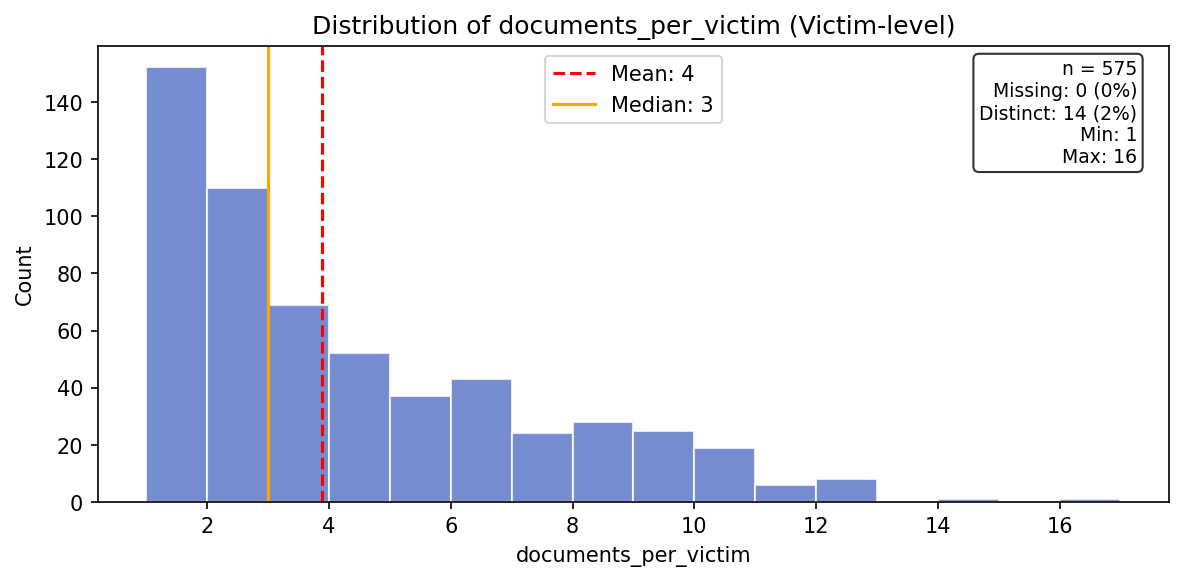
\includegraphics[width=0.8\textwidth]{plots/descriptive_statistics/document_count_distribution_by_victim.png}
    \caption{Distribution of document counts per victim.}
    \label{fig:document_count_distribution}
    \end{figure}
    
    \begin{figure}[tbp]
    \centering
    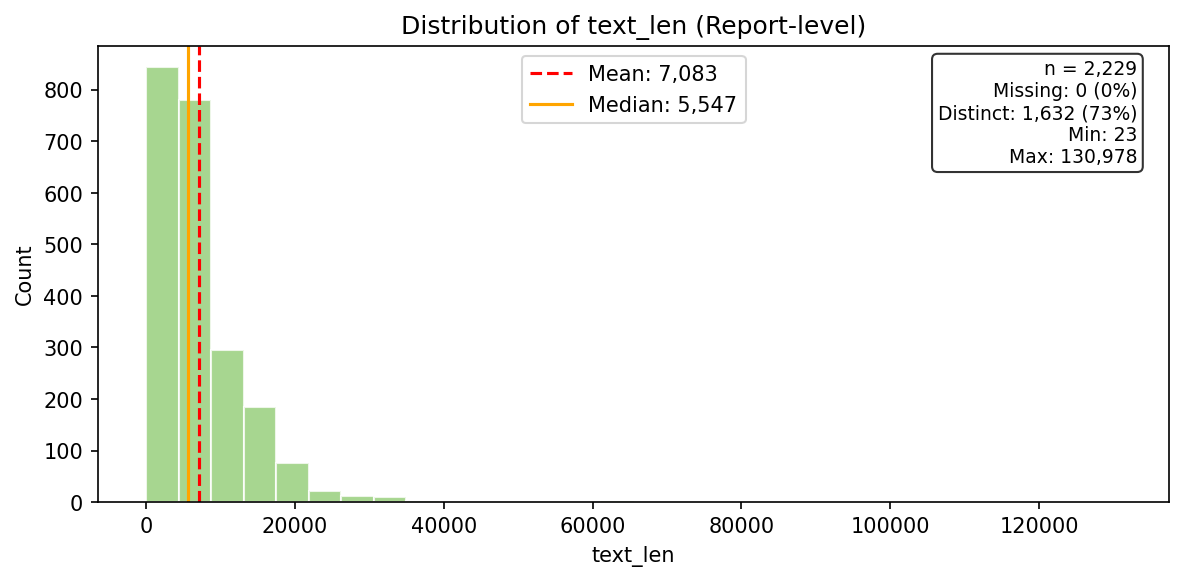
\includegraphics[width=0.8\textwidth]{plots/descriptive_statistics/text_length_distribution_by_report.png}
    \caption{Distribution of text length per report.}
    \label{fig:text_length_distribution}
    \end{figure}
    


The codebook itself is extensive, spanning seven sections that cover victim demographics, circumstances of capture, outcome of the disappearance, perpetrator characteristics, judicial proceedings, and observational comments, with several dozen substantive coded variables in total. Not all victims in the corpus have annotations for every coded field. A substantial portion records free text descriptions, dates, or geographic identifiers that cannot be used directly in a classification-based evaluation. Among the categorical fields that remain, many encode details that are specific to a narrow research domain, such as the identity of individual organized crime groups or the type of judicial sentence.  The codebook used by the original human coders instructed them to enter 999 when no information was available in the news articles, and as a result many labels carry high rates of missing values across the 575 victims. The degree of missing values varies substantially from one label to another, depending on whether the coder was able to find the information in the news articles for the given victim.

For this study, we select a subset of categorical labels that have relatively low rates of missing values and that capture information relevant to a broad audience rather than to a single specialized subfield.

Three labels meet these criteria. The variable / colum \emph{Desenlace} records the outcome of the disappearance as reported in the press. Of the 575 victims, 393 have an annotation for this field, and the distribution across its seven original categories is heavily concentrated: 254 victims are recorded as still disappeared and 91 as found dead, while the remaining five categories, including liberation by captors or authorities, found alive, self-liberation, and found without specification of condition, each contain fewer than 25 cases as shown in Figure~\ref{fig:desenlace_distribution}. \emph{Captura tipo} records the type of place where the victim was captured, using place categories from the HURIDOCS micro-thesaurus. This field has 243 annotated victims and eight original categories, with the two most frequent being means and routes of transport and places of connection at 90 cases and places related to the victim such as the home or workplace at 81, while the remaining six categories range from 1 to 28 cases as shown in Figure~\ref{fig:captura_tipo_distribution}. \emph{Vic grupo} social records the social group to which the victim belongs. This field has 273 annotated victims and ten original categories, with the most frequent being people who work in service industries at 95 cases, followed by civil servants at 49 and students at 45, and smaller counts for professionals, activists, people associated with politics, organized crime, land workers, and others as shown in Figure~\ref{fig:vic_grupo_social_distribution}.

\begin{figure}[tbp]
\centering
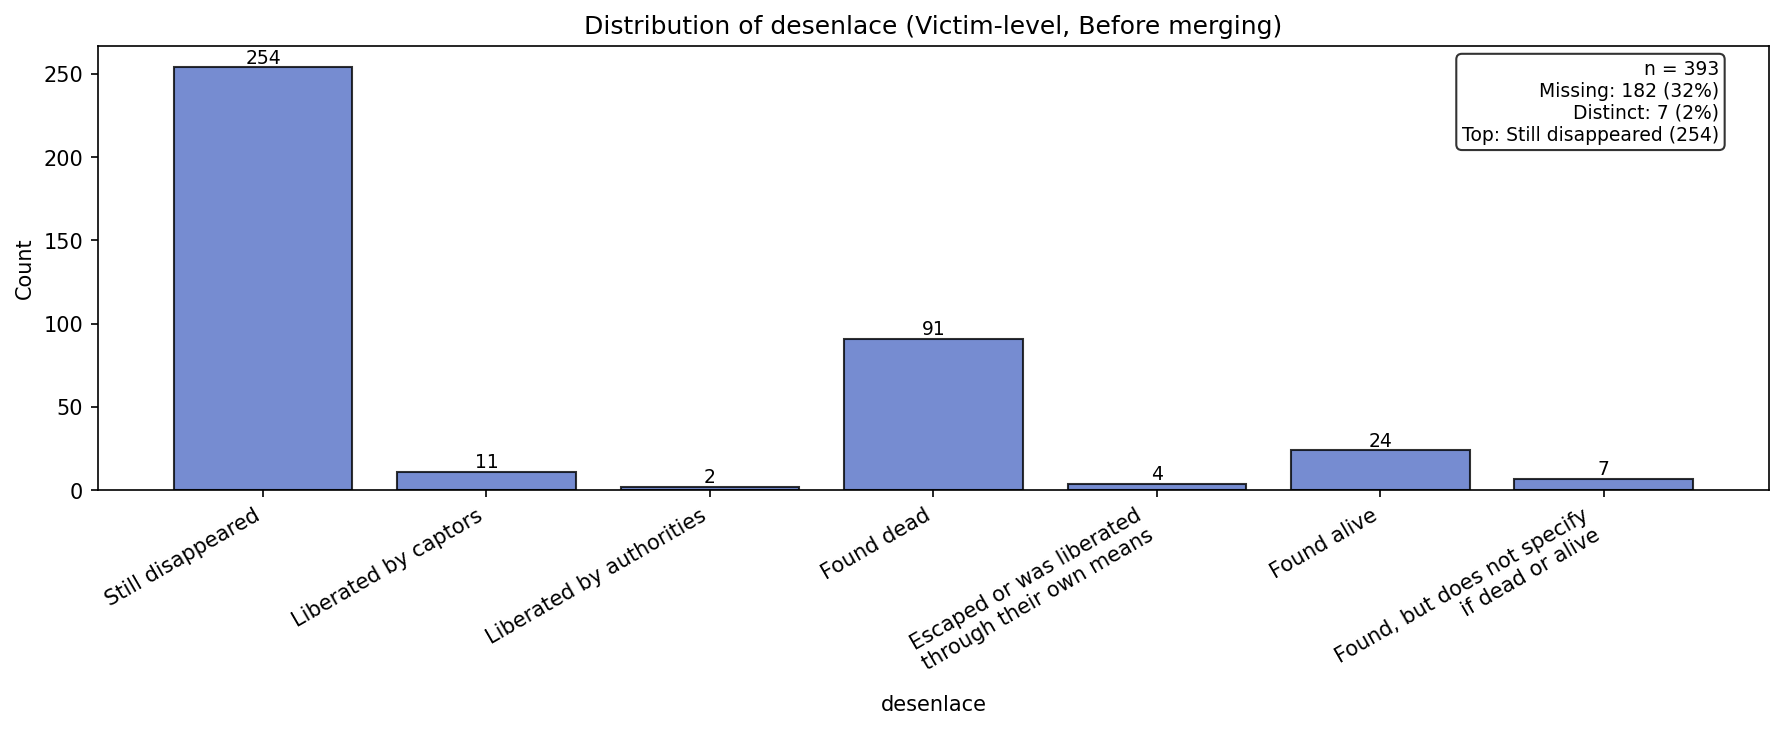
\includegraphics[width=0.8\textwidth]{plots/descriptive_statistics/desenlace_distribution_by_victim_before_merging.png}
\caption{Distribution of desenlace categories per victim before merging.}
\label{fig:desenlace_distribution}
\end{figure}

\begin{figure}[htbp]
\centering
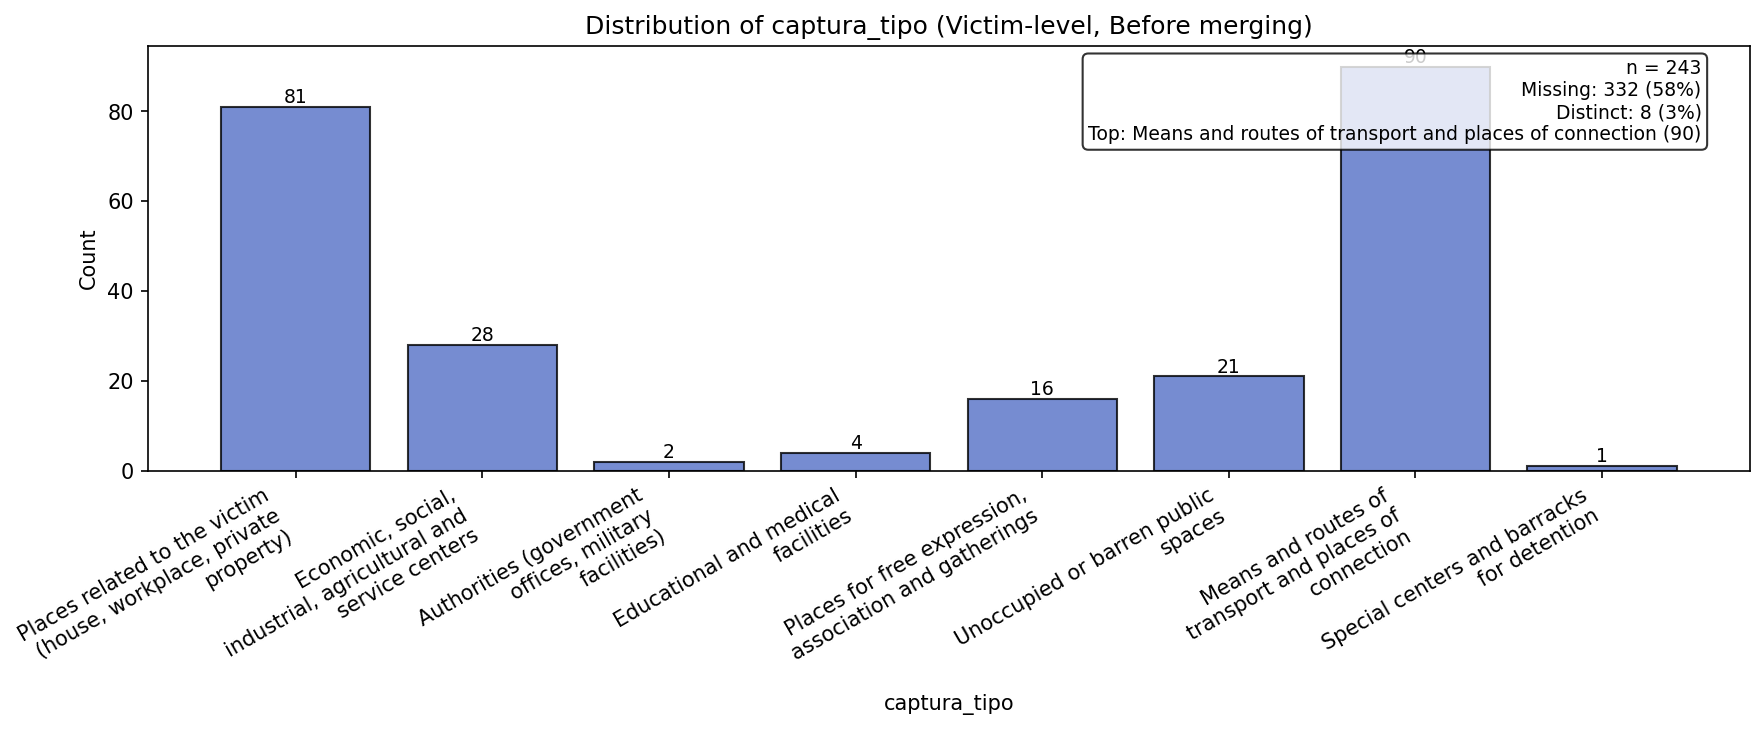
\includegraphics[width=0.8\textwidth]{plots/descriptive_statistics/captura_tipo_distribution_by_victim_before_merging.png}
\caption{Distribution of captura tipo categories per victim before merging.}
\label{fig:captura_tipo_distribution}
\end{figure}

\begin{figure}[tbp]
\centering
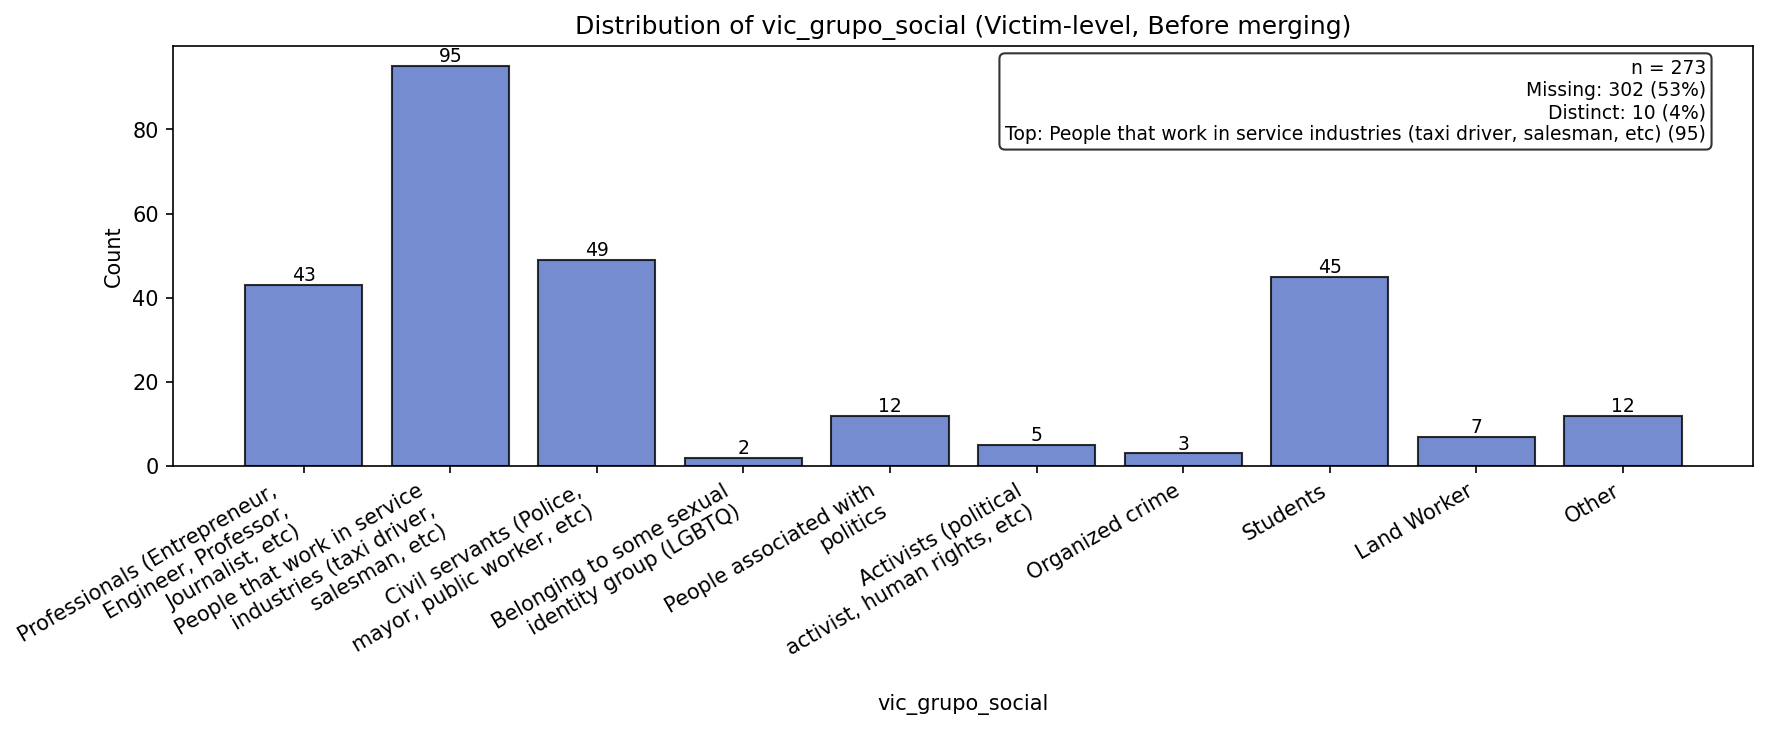
\includegraphics[width=0.8\textwidth]{plots/descriptive_statistics/vic_grupo_social_distribution_by_victim_before_merging.png}
\caption{Distribution of vic grupo social categories per victim before merging.}
\label{fig:vic_grupo_social_distribution}
\end{figure}


\subsection{Challenges in the Data}\label{challenges-in-the-data}

\subsubsection{Scraped File Errors}\label{scraped-file-errors}

The scraped corpus contains three categories of textual noise in the web scraping process: 
\begin{description}
    \item[HTTP error pages / missing pages:] target URL was unreachable
    \item[Ancillary or obscured text on pages:] website with
    extraneous information such as navigation menus, footers, and
    advertising banners interleaved with the article body, obscuring the
    relevant text.
    \item[Irrelevant content:]  content that is
topically adjacent but are substantially irrelevant, such as suggested
article previews or user comment threads appended to the original
report.
\end{description}
 
Each of these error types introduces noise that can mislead or
degrade downstream text processing. Each error type has consequences for downstream tasks such as fine-tuning based on a noisy corpus.\footnote{Error pages yield no usable content, causing the model to process an empty or irrelevant document as if it were a valid report when the document or victim was linked to a set of annotations, which can establish a false connection
between the the annotation and empty documents. Page elements such as
navigation menus and footers inflate the input with structurally
irrelevant text, increasing context length while contributing no article
content.} When a model is fine-tuned on such documents, the training
signal is distributed across the full input including the noise, making
it difficult for the model to learn which spans are responsible for a
given label. Distractive content such as suggested articles or comment
threads poses a more subtle but more dangerous risk, as the text is
topically connected to disappearance reporting and can cause the model
to attribute information from unrelated cases to the victim under
analysis, resulting in hallucinated or incorrectly sourced output.

To address these noise sources, the authors attempted to rescrape
the original URLs to obtain cleaner versions of the documents. However,
a portion of the original URLs were no longer accessible at the time of
rescraping. For those that remained available, the structural issues
persisted, as the noise originates from the design of the source
websites themselves rather than from the scraping process. Navigation
menus, comment sections, and related article modules are integral parts
of the page layout and are captured by any general-purpose scraper that
retrieves the full page body.

The authors also attempted rule-based preprocessing to remove known
sources of noise, targeting HTML tags, residual markup, and other
structural elements. While this reduced formatting noise, it could not
reliably eliminate all types of errors such as navigation text or other
irrelevant information, because each webpage were designed differently.
As for related content such as suggested articles or comment threads
which appear as valid plain text, are almost indistinguishable from
article content by pattern-matching rules. Processing them requires
substantive human hours and is not scalable. Approaches such as optical
character recognition (OCR), which convert image-based documents to
machine-readable text, are not applicable here, as the documents were
already scraped as plain text. The noise in this corpus is not a
accessibility problem but a content boundary or scope problem, and no
rule-based or format-conversion method can reliably locate where the
article body ends and extraneous content begins without semantic
understanding of the text.

\subsubsection{Ambiguity for
Classification}\label{ambiguity-for-classification}

A second category of challenge arises from the inherent ambiguity of the
context described in the news text itself. Real-world entities and
places do not belong to a single category by nature, and the language
used to describe them reflects this multiplicity. For example, a bus
route office in a residential area is simultaneously a commercial
service facility and a place in close proximity to where the victim
lived. The news report does not resolve this ambiguity, for its purpose
is to report the event, not to decide how to classify the event. In this
case, because the news text does not distinguish between these
dimensions, both interpretations are equally supported by the available
evidence. When the model and the human annotator arrive at different
valid categories from the same text, the evaluation records a false
negative even though neither answer is wrong. The disagreement
originates in the indeterminacy of the source text, not in a failure of
the model or the annotation.

Evaluating against fine-grained categories that each case is expected to
match a single label penalizes valid model outputs that approaches the
text from a different but equally defensible understanding of the same
text. To produce an evaluation that is less sensitive to this inherent
ambiguity, the original categories were collapsed into broader groupings
that reduce the number of cases where two valid answers fall into
different classes.

\section{Method}\label{method}

% DEFINE THE TASKS!  THEN HOW THEY ARE ACCOMPLISHED.

This method addresses a unit of analysis mismatch between victim level annotations and document level source reports. The task is to reuse the existing codebook and human annotations by aligning them with the original texts, extracting source grounded evidence for each coded field, producing clean structured document level summaries, and updating those summaries across multiple reports while preserving traceability to the supporting spans. The following subsections explain how each of these tasks is implemented.

\subsection{Task Definitions}\label{task-definitions}

The task is to transform a set of messy, multi document
news reports associated with a single victim into a structured, evidence
traceable document level representation that supports reuse of the
existing codebook and annotations.

Another critical requirement is that the output text must be noise-free,
so that any further LLM tasks can be meaningful. The text must combine
extraction of verbatim spans with structured aggregation across
documents, so that the resulting representation is both clean enough to
serve as LLM input and anchored tightly enough to the source material to
support reuse of the existing coded data and codebook definitions.


\subsection{Model Setup}\label{model-setup}

All LLM calls were executed using instruction tuned models served through vLLM~\cite{Kwon_etal2023}. The default configuration uses the AWQ INT4 quantized Meta Llama 3.1 8B Instruct model~\cite{Dubey_etal2024}, and cross model comparisons use Meta Llama 3.1 70B Instruct, Gemma 3 12B IT~\cite{GemmaTeam2025}, and Ministral 3 8B Instruct~\cite{MistralAI2026}. We use deterministic decoding with temperature 0.0. Generation is capped at 1024 tokens for summarization and 256 tokens for classification, and outputs are constrained to a fixed JSON schema to produce consistent structured fields for extracted spans and label predictions.

\subsection{Unit of Analysis}\label{unit-of-analysis}

On the dataset side, the original dataset was coded with the victim as
the unit of analysis. To be specific, human coders annotated features
about each kidnapping victim such as method of capture, who carried out
the threats, how the person was captured etc. The annotations are
structured around victim records.

On the source data side, the original scraped reports were organized by
documents. A single victim may appear across multiple documents, and
those documents were collected by news source or origin, not by victim.
However, the annotations were made at the victim level, not the document
level, and the knowledge between the annotations and the source data is
not realistically recoverable by human labor.

On the downstream task side, the downstream tasks may include
fine-tuning, annotation or classifications for other reports that domain
experts might gathered, so the output must be organized and labeled in a
way that can be directly consumed by an LLM or classifier operating on
individual documents, document level preferably. However, the original
annotations were not coded at the document level, so it is unclear which
document should carry which annotation. For example, a victim's method
of capture may be mentioned in one document while the identity of who
carried out the threats appears in another, yet both were annotated at
the victim level, without reference to a specific document. If
victim-level annotations are simply propagated down to the document
level, future LLM training tasks will receive incorrect signals, as each
document would be labeled with information it does not necessarily
contain.

\subsection{Extraction vs
Summarization}\label{extraction-vs-summarization}

As stated above, another requirement for the dataset for this set of
tasks is that the annotations from prior human coders remain connected
to the source texts, so that the coded features can be traced back to
the original documents and reused without re-annotation. Even though
recreating the human annotation is almost impossible and unrealistic,
with the help of LLMs, we now can extract the exact spans of the text
where the decision of annotations were made and record them as evidence.
This allows researchers to trace the source of the information rather
than having an annotation to victim link without knowing where, how and
why they were annotated that way.

Given the above requirements, the process cannot rely on generative
summarization alone, which might condenses and paraphrases and breaks
the link to the original evidence.

\subsection{Pipeline}\label{pipeline}

The pipeline takes each victim's documents one at a time in sequence,
extracting relevant spans, generating a label-structured summary
anchored to those spans, and updating the summaries using previous
summaries as context. This pipeline satisfies the task definition by
producing document level outputs that are clean enough for downstream
language model use while keeping each coded field traceable to evidence
in the original documents.

\subsubsection{Extraction of evidence}\label{extraction-of-evidence}

In the first step of the pipeline, we extract evidence rather than only
generating a paraphrased summary. For each input document, the model is
instructed to return verbatim text spans for each item in the codebook
schema, producing a structured evidence record keyed by label. This
creates traceability because every coded field is paired with the exact
source phrase that supports it, so downstream users can verify where the
information came from in the original report. The evidence output is
designed to demonstrate that the link between each annotation and its
source text is preserved and can later be verified, and it also includes
a character index that locates each span within the document text. This
index records how many characters into the document the extracted span
begins, so a future researcher can find the exact spot in the original
text and confirm the evidence.

\subsubsection{Summarization with Context and
Evidence}\label{summarization-with-context-and-evidence}

In the second step of the workflow, we generate a coherent summary while
keeping it anchored to evidence and guided by the codebook schema. The
model is given the document text together with the label definitions
that specify the meaning of the labels and how the human coders would
code the information, and it is also provided with the extracted span
structure so that each sentence or clause of the summary can be linked
back to the corresponding evidence. For example, the first sentence may
be about the victim, and the second sentence may be about the method of
capture, and the third sentence may be about who carried out the
threats, instead of condensing the information into a single sentence
where all the information is mixed together. This makes the summary
different from vanilla summarization because it is not an unconstrained
paraphrase of the document, rather, with the paragraph structured label
by label, it will be easier for an LLM to pick up the right information.
At this stage, summarization is performed at the level of a single
document and is designed to be clean, structured, and directly usable
for downstream models.

\subsubsection{Updating Summary with
state}\label{updating-summary-with-state}

In a typical single request, an LLM is stateless, meaning that it does
not retain information from earlier calls, but our workflow preserves
memory by maintaining an explicit conversation state for each victim as
their documents are processed. The workflow maintains an explicit
conversation state for each victim that accumulates across documents as
they are processed sequentially. The prompt instructs the model to check
each new document against the existing summary and update only the
fields where new information is found. If a document contains no
relevant information, the runner keeps the previous summary unchanged
rather than replacing it with the model's output. Each turn also records
the output of that turn, preserving what was extracted and what summary
was produced at that step for later inspection and reuse. When a
document contains no relevant information, the workflow avoids replacing
the existing running summary, so the accumulated context is not lost as
the sequence progresses.

\section{Evaluation and Results}\label{eval_results}

Evaluation of summarization tasks compares the
text summary with a gold standard reference text. Given the messy and noisy initial documents, it is difficult to
use them as reference texts.  The prior work has human
annotations classifying the information in the 
summary text. The evaluation tests whether generated summaries reproduce
the same labels as the human annotations, comparing a simple
summarization baseline against the proposed method, across major model
families, and across model sizes.

\subsubsection{Human Gold Standard}\label{human-gold-standard}

Many existing summarization evaluation methods require a gold standard reference text against which generated summaries can be compared using similarity metrics. Because the source documents in this dataset are themselves messy and noisy, they cannot serve as reliable reference texts, and there are no clean human-written reference summaries for this corpus. Should the research use these documents as reference texts, the output generated from original text will be heavily influenced by the noise, so that the difference between the result of original text and the result from cleaned summaries will be inflated, making the evaluation not reliable. However, the data set contains human annotations coded at the victim level, and these annotations are used as ground truth. Evaluation proceeds by classifying the generated summary text and comparing the resulting labels against the human annotations, testing whether the summaries preserve the same information that human coders recorded. 

Another issue discussed above is that the original codebook contains fine-grained categories. One example is that the method of capture can be distinguished into general kidnappings and special type kidnappings such as Levantón. Without external context plugged in, or making the model fine-tuned on the specific context, it will be difficult for LLM models to distinguish between the two.


The second issue about the fine-grained categories is that some of the source texts themselves are ambiguous, where a single entity or event can validly map to more than one category, even though both answers can be defensible. In such a case, the model and the human coder may generate different results, even though both may capture the same spans. And even for the models themselves, run on ambiguous texts, can lead to different results even parameters are fixed. One typical example of the text ambiguity is the bus station. It is both an infrastructure that holds high economic value, and a place in close proximity to where the victim lived. Due to these nature of the text, the performance might be greatly reduced if not properly handled. To reduce the number of categories where multiple valid answers fall into different classes, the original categories are collapsed into broader groupings before evaluation. The detailed distribution of the collapsed categories is shown in Figure~\ref{fig:desenlace_distribution_after}, Figure~\ref{fig:captura_tipo_distribution_after}, and Figure~\ref{fig:vic_grupo_social_distribution_after}.

\begin{figure}[htbp]
\centering
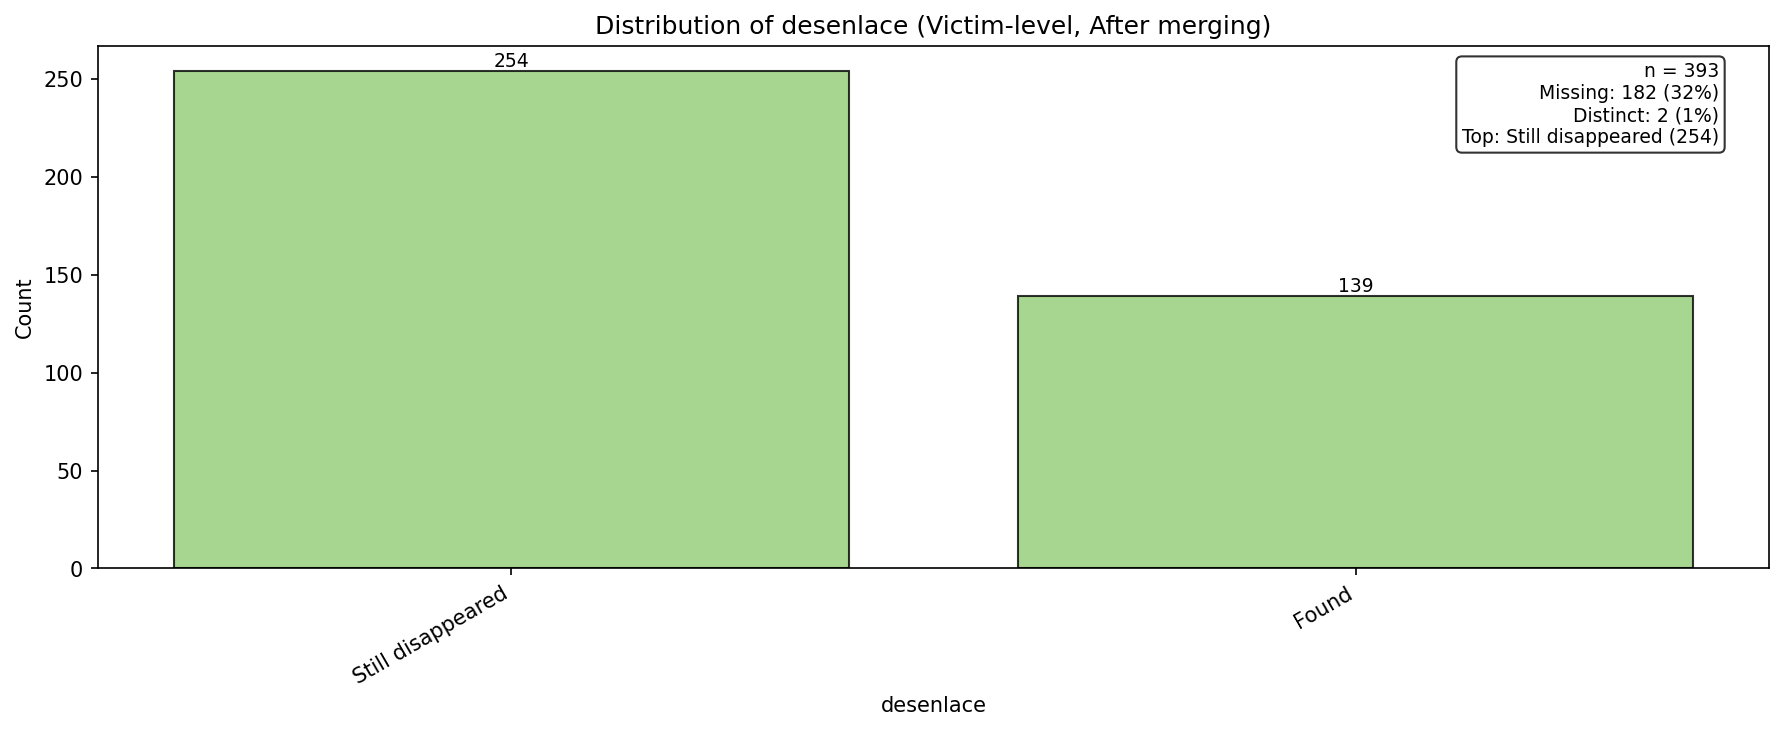
\includegraphics[width=0.8\textwidth]{plots/descriptive_statistics/desenlace_distribution_by_victim_after_merging.png}
\caption{Distribution of desenlace categories per victim after merging.}
\label{fig:desenlace_distribution_after}
\end{figure}

\begin{figure}[htbp]
\centering
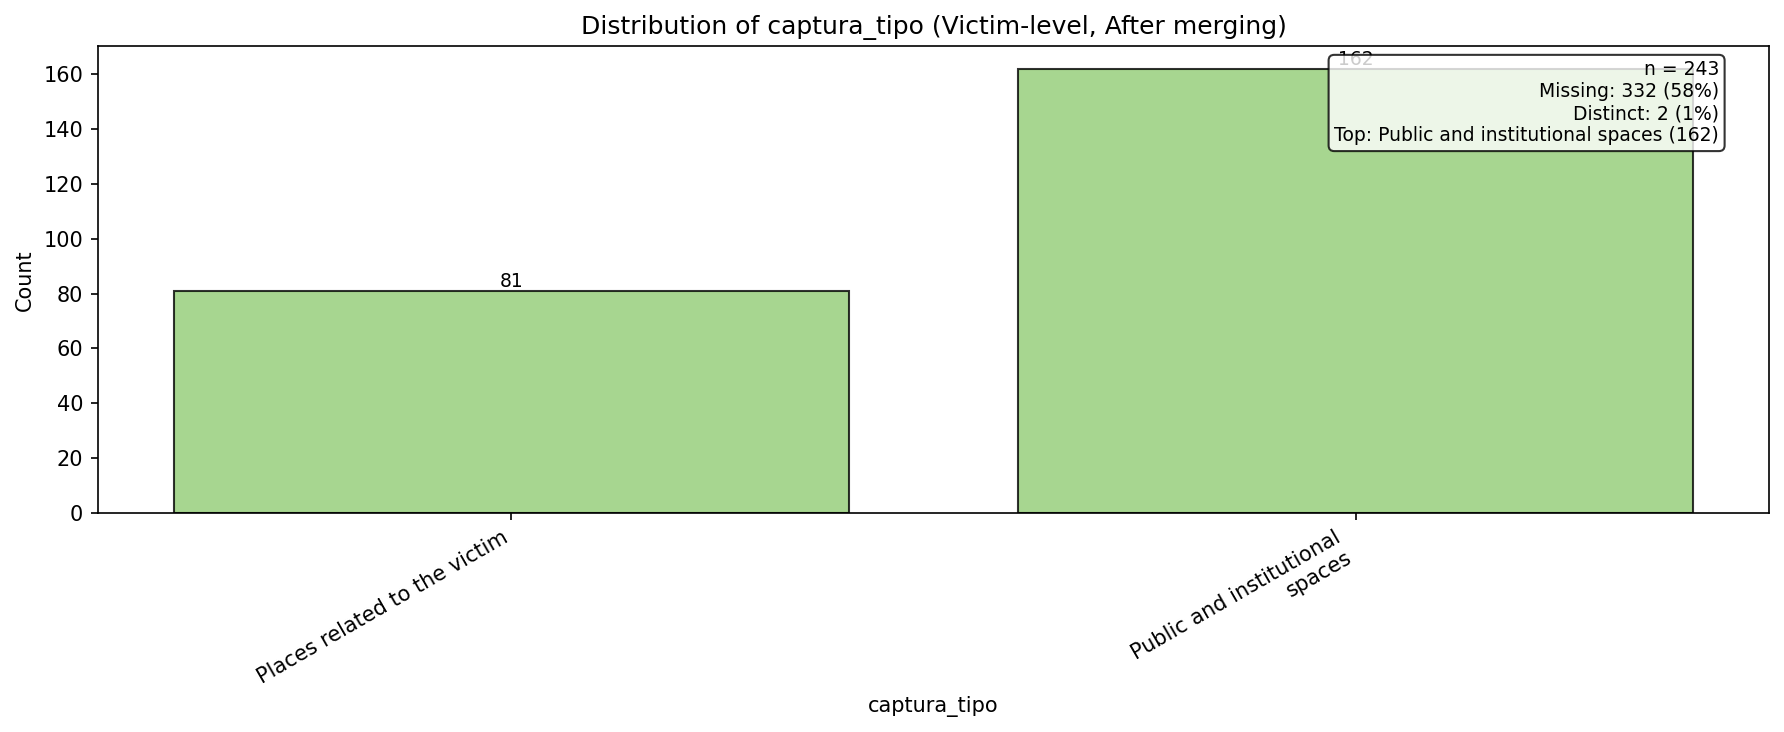
\includegraphics[width=0.8\textwidth]{plots/descriptive_statistics/captura_tipo_distribution_by_victim_after_merging.png}
\caption{Distribution of captura tipo categories per victim after merging.}
\label{fig:captura_tipo_distribution_after}
\end{figure}

\begin{figure}[htbp]
\centering
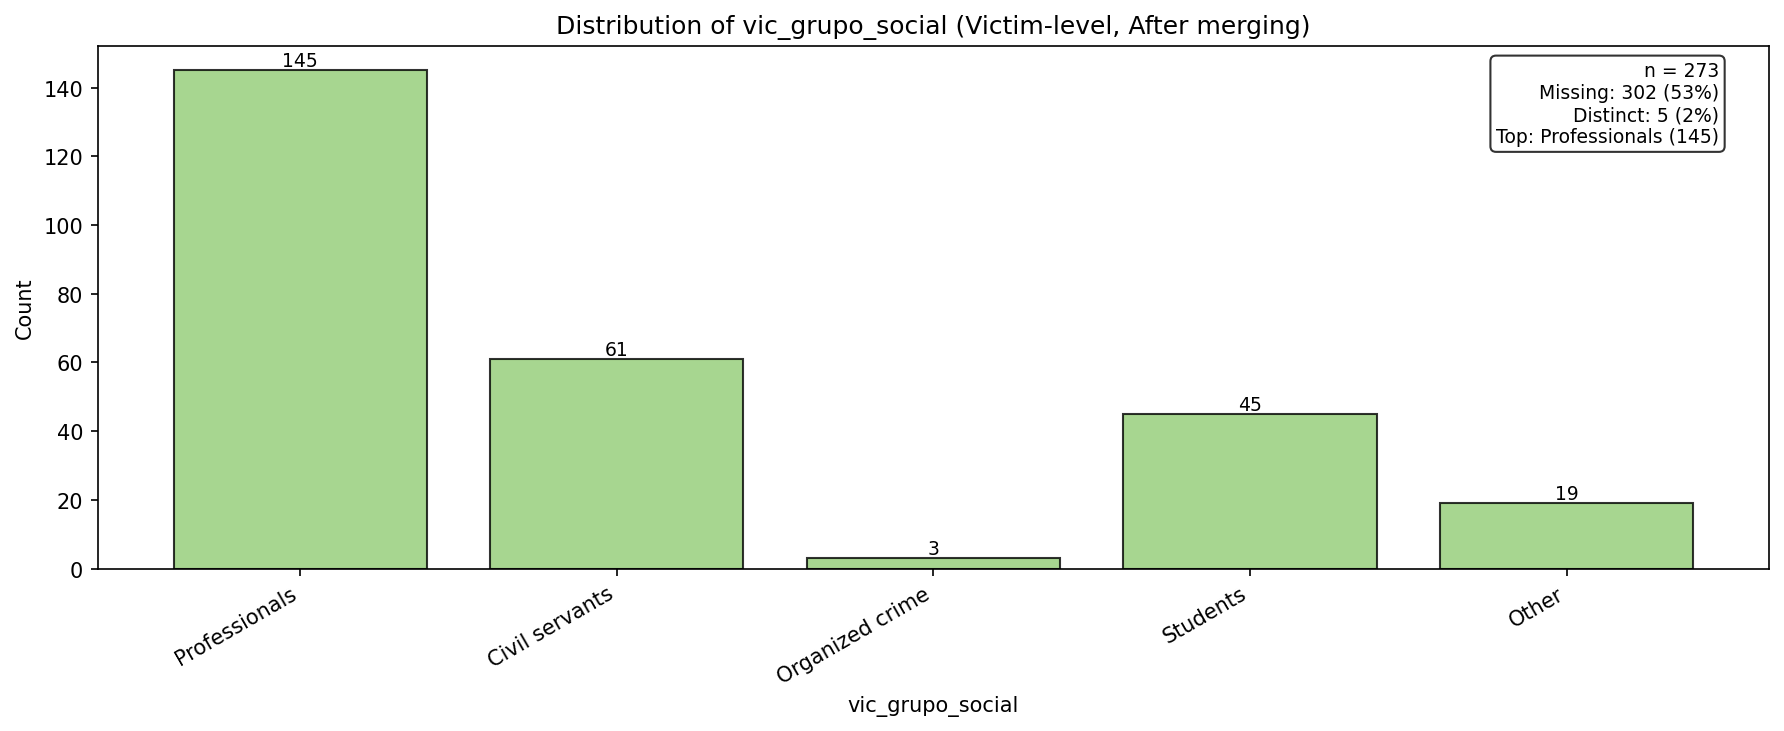
\includegraphics[width=0.8\textwidth]{plots/descriptive_statistics/vic_grupo_social_distribution_by_victim_after_merging.png}
\caption{Distribution of vic grupo social categories per victim after merging.}
\label{fig:vic_grupo_social_distribution_after}
\end{figure}

Another issue of the human annotations is the lost documents. Many of the decisions were made when the human coders were able to access more documents than we currently can fetch, either from their sources or from the internet. This means that some of the annotations are not supported by the documents that are available to us. To address this issue, we need to select the annotations that are supported by the documents that are available to us. This is also critical for the goal of this project, which is to relink the annotations to the source text and make them usable for downstream tasks.

\subsubsection{LLM as Evaluators}\label{llm-as-evaluators}

Recent work has proposed LLM-as-judge evaluators for summarization that compare a generated summary directly against its source text rather than against a human reference summary. SummaC treats factual consistency as a source grounding problem and uses natural language inference over smaller units of the source and the summary to estimate whether the content of the summary is supported by the original document~\cite{Laban_etal2022}. G-Eval uses a large language model as a judge and asks it to score generated output through structured prompts and intermediate reasoning steps~\cite{Liu_etal2023}. These methods are useful because they move evaluation away from surface similarity and toward the question of whether a summary remains faithful to the source.

In our setting, however, these methods are difficult to use in a meaningful way because the source reports are themselves messy, noisy, and often mixed with irrelevant but topically related material. A source to summary consistency score may therefore reward a system for preserving noise, or penalize a cleaned and focused summary for leaving out distractive content that should not be carried forward. For that reason, these evaluator scores alone cannot answer the main question of this paper. The more informative comparison is between directly generated summarization from the messy reports and the structured extractive summary from the proposed method, because this shows whether the structured extractive pipeline preserves the information needed for downstream coding better than a simpler generative baseline under the actual conditions of this corpus.

\subsubsection{Hallucination Evaluation
}\label{hallucination-evaluation-literature}

Beyond evaluation on performance, the hallucination evaluation literature provides an important metric for LLMs in computational social science in a broader sense. The most relevant problem here is input conflicting hallucination, where generated content is not supported by the source text. This is the central risk for our task because the model is asked to extract and summarize information from noisy documents rather than answer open domain questions from background knowledge. However, given tha nature of our input text, the hallucination evaluation is not as straightforward as the ones in the literature.

Recent literature generally groups evaluation methods into human evaluation, model based evaluation, and rule based evaluation~\cite{Zhang_etal2025}. Human evaluation remains the most reliable because annotators can examine whether each generated claim is supported, unsupported, or irrelevant with respect to the source text~\cite{Min_etal2023}. However, given the purpose of our task, the human evaluation does not solve the problem shared with human coder.

LLM based methods then approximate this process in different ways. Large Language Models (LLMs) based methods use an evaluator model to judge factual consistency between the source and the output, sometimes with retrieved evidence~\cite{Liu_etal2023}, while rule based methods use structured comparisons such as question answering over the source and the summary, textual entailment style checks, named entity based comparisons, or source grounded reference contrasts~\cite{Laban_etal2022,Lee_etal2022}.

Hallucination evaluation matters in our project because the outcome of the proposed method is extractive summarization that should preserve the information from the source text while leaving out the noise. The generation part opens up the risk of hallucination, so evaluation of hallucination is necessary to ensure the quality of the output~\cite{Zhang_etal2025}.

This is not only a language quality issue but also critical for downstream tasks. In political science and computational social science setups, unsupported or even entirely fabricated generated details can change coded variables, weaken traceability, and distort substantive conclusions. A careful evaluation of hallucination therefore contributes to the field by making LLM based extraction more transparent, more reproducible, and more defensible as empirical evidence.

\section{Results}\label{results}

\begin{figure}[htbp]
\centering
\begin{minipage}{0.32\textwidth}
\centering
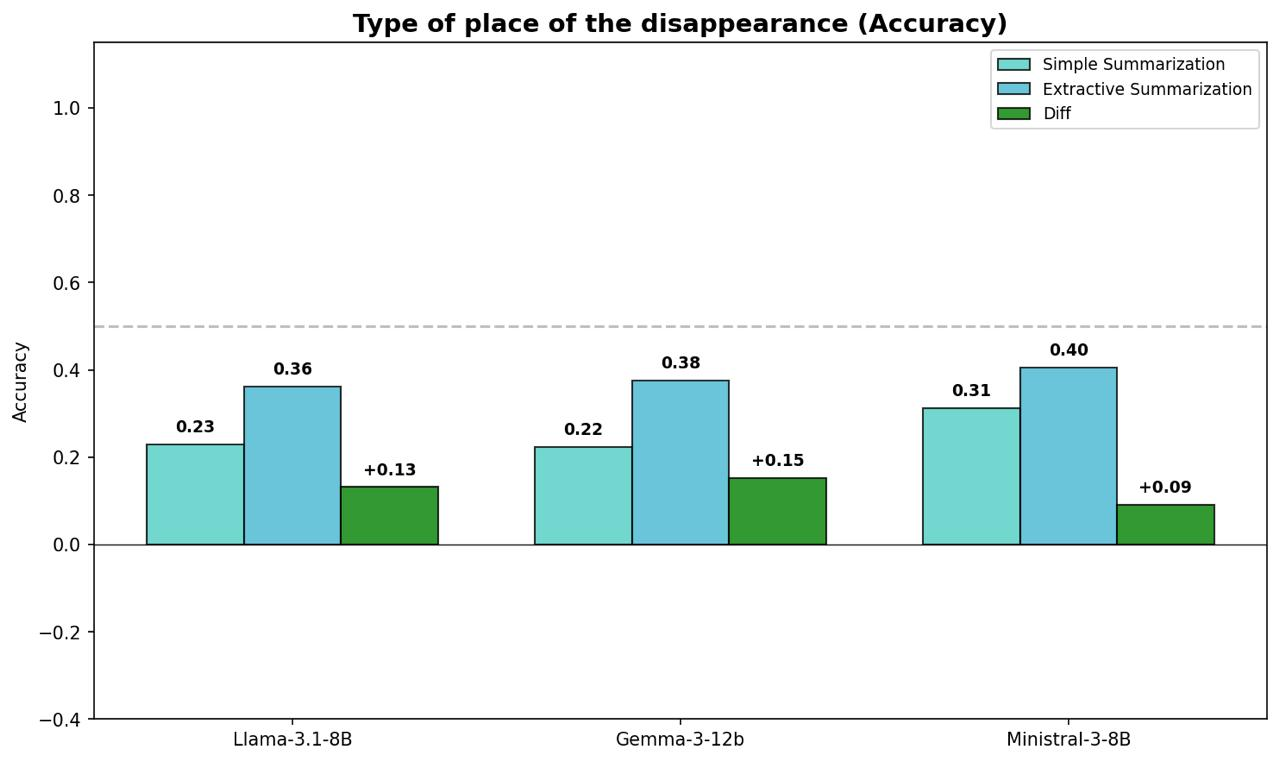
\includegraphics[width=\textwidth]{plots/evaluation/benchmarks/less_labels_multi_models/metrics_captura_tipo.png}
\end{minipage}
\hfill
\begin{minipage}{0.32\textwidth}
\centering
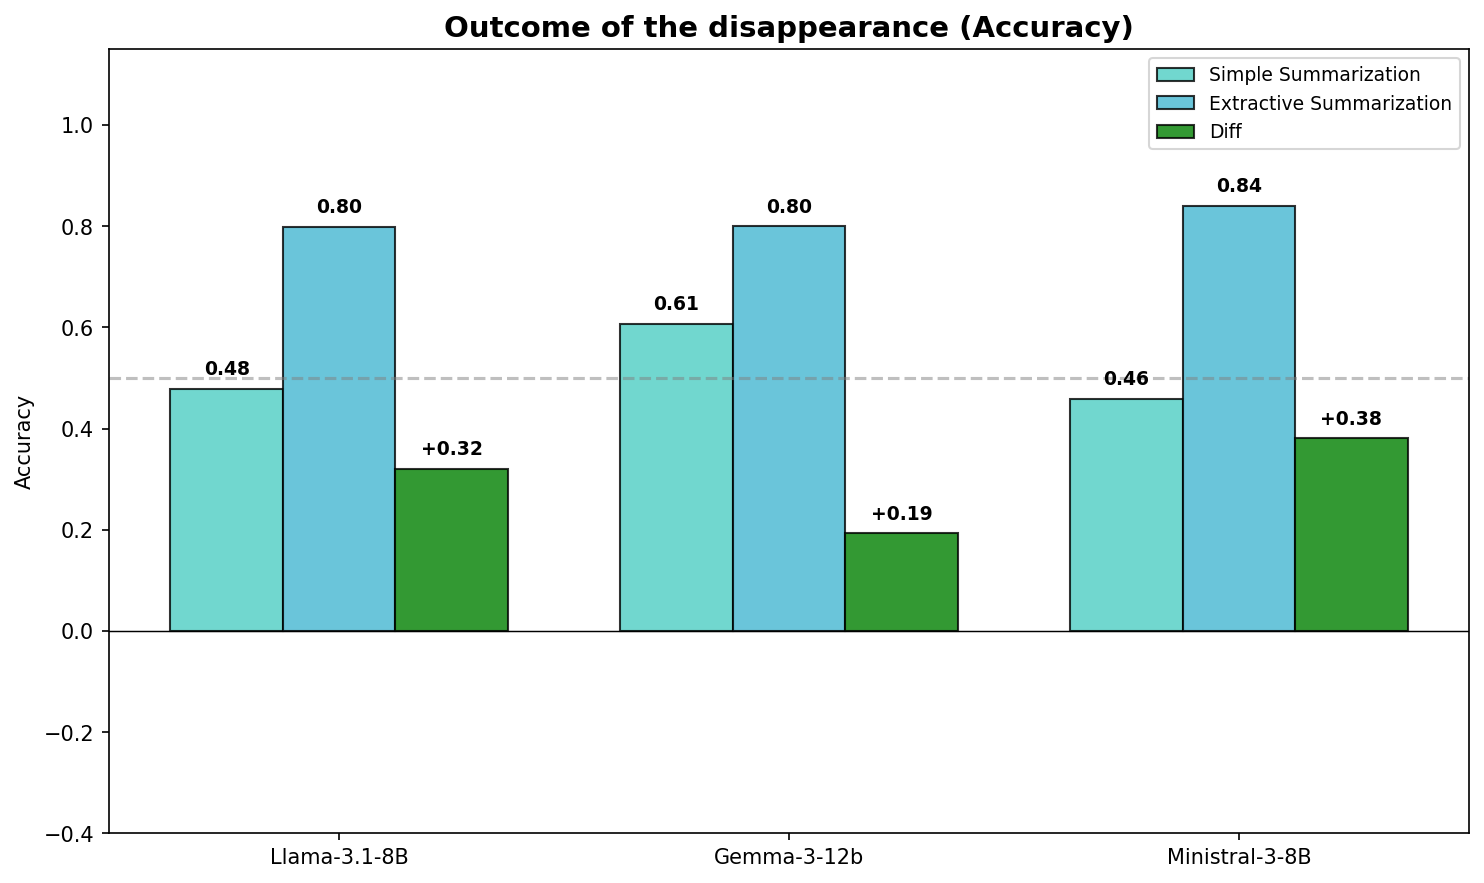
\includegraphics[width=\textwidth]{plots/evaluation/benchmarks/less_labels_multi_models/metrics_desenlace.png}
\end{minipage}
\hfill
\begin{minipage}{0.32\textwidth}
\centering
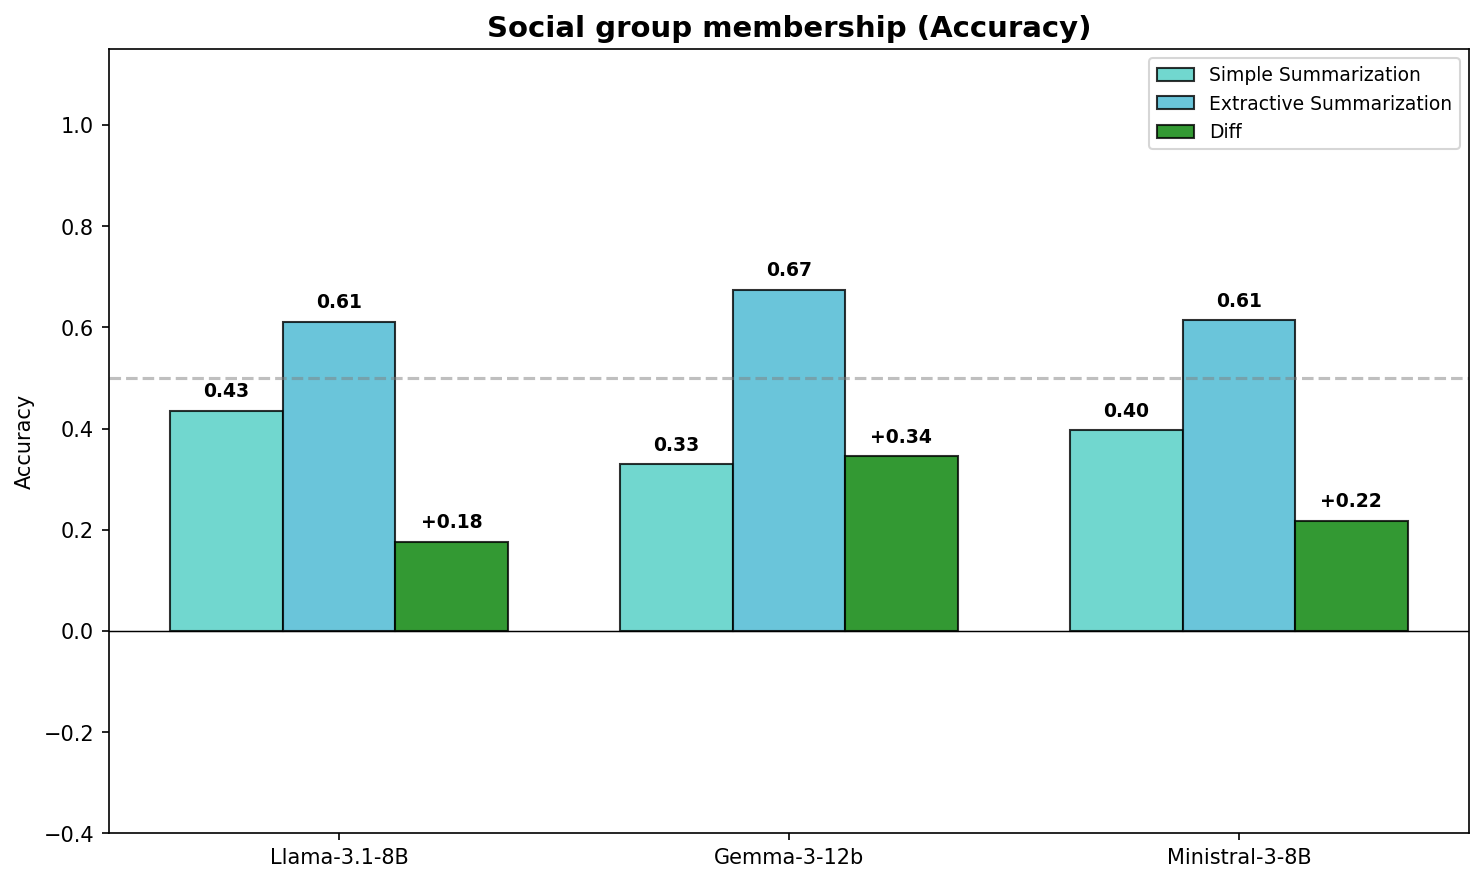
\includegraphics[width=\textwidth]{plots/evaluation/benchmarks/less_labels_multi_models/metrics_vic_grupo_social.png}
\end{minipage}
\caption{Classification metrics by label across models (collapsed categories). Left: captura tipo. Center: desenlace. Right: vic grupo social.}
\label{fig:metrics_by_label}
\end{figure}

\subsection{Baseline vs Proposed
Method}\label{baseline-vs-proposed-method}

The baseline for this evaluation is a simple summarization approach that generates a direct summary of each victim's documents without codebook guidance or structured extraction. The proposed method instead uses the codebook schema to guide extraction and produces label-structured summaries anchored to verbatim evidence spans. Each panel in Figure~\ref{fig:metrics_by_label} compares these two approaches on one of the three selected labels, reporting the classification accuracy of the simple summarization baseline, the extractive summarization method, and the difference between them. Across all three labels and all three models, the proposed method consistently outperforms the baseline, with every difference value being positive. The improvement is largest for outcome, where extractive accuracy reaches 0.80 to 0.84 compared to 0.46 to 0.61 for the baseline, yielding gains between +0.19 and +0.38. Social group shows similarly substantial gains, rising from a baseline range of 0.33 to 0.43 to an extractive range of 0.61 to 0.67. Type of place of capture remains the most difficult label for all models, with extractive accuracy between 0.36 and 0.40, but even here the proposed method improves over the baseline by +0.09 to +0.15. These results indicate that codebook-guided extraction produces summaries that preserve the information needed for downstream classification more reliably than unconstrained summarization across all labels evaluated.

\subsection{Model Comparisons}\label{model-comparisons}

Figure~\ref{fig:metrics_by_label} also allows a cross-model comparison, since each panel shows all three models side by side on the same label. All three models follow the same pattern: the proposed extractive method outperforms the simple summarization baseline on every label, and no model fails to benefit from the structured workflow. At the same time, the models differ in where they show the largest gains. Gemma 12B achieves its strongest improvement on social group, rising from 0.33 to 0.67 for a gain of +0.34, while Ministral 8B shows its largest gain on outcome, rising from 0.46 to 0.84 for a gain of +0.38. Llama 8B falls between the two, with its largest gain also on outcome at +0.32. For type of place of capture, all three models remain below 0.40 even with extractive summarization, confirming that this is the most difficult label to classify regardless of which model is used. The consistency of the improvement across all three model families suggests that the performance gain originates in the workflow design rather than in the capability of any single model.

The three models also span a range of parameter counts, with Llama 3.1 8B and Ministral 3 8B at 8 billion parameters and Gemma 3 12B at 12 billion. Despite this difference, Gemma does not uniformly outperform the two smaller models. Ministral 8B achieves the highest extractive accuracy on outcome at 0.84 and on type of place of capture at 0.40, while Llama 8B and Ministral 8B both reach 0.61 on social group compared to 0.67 for Gemma. The 4 billion parameter gap does not produce a consistent advantage on any label, which suggests that within the 8B to 12B range the proposed workflow provides comparable benefits regardless of model size.

\subsection{Annotation to Documents Mapping}\label{annotation-to-documents-mapping}

Beyond classification accuracy, a central question for this pipeline is whether the original human annotations can be traced back to evidence in the available source documents and, where they cannot, whether the constraint is the state of the archive rather than the quality of extraction.

\begin{figure}[htbp]
\centering
\begin{minipage}{0.32\textwidth}
\centering

\includegraphics[width=\textwidth]{plots/evaluation/matching/less_labels_multi_models/cumulative_support_curve.png}
\end{minipage}
\hfill
\begin{minipage}{0.32\textwidth}
\centering
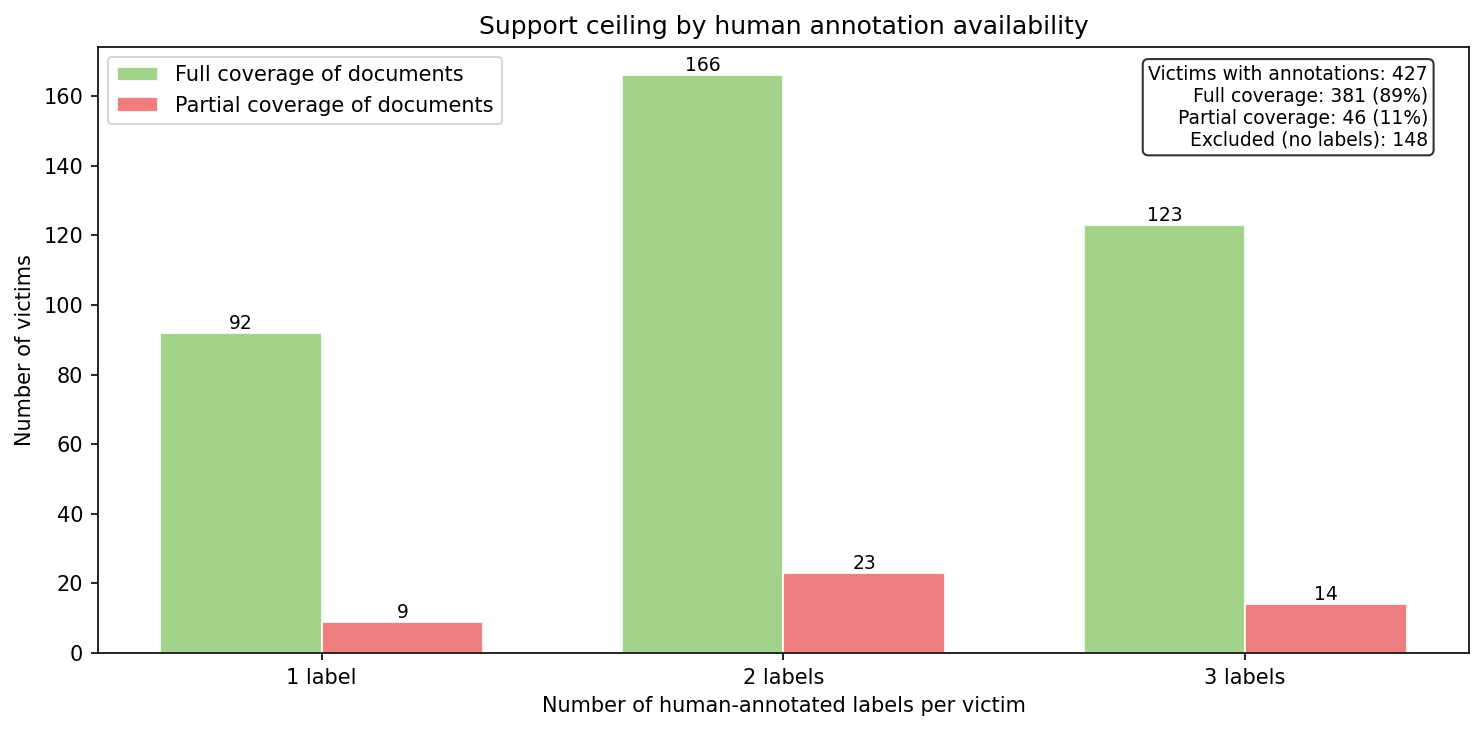
\includegraphics[width=\textwidth]{plots/evaluation/matching/less_labels_multi_models/support_ceiling_by_annotation_availability.png}
\end{minipage}
\hfill
\begin{minipage}{0.32\textwidth}
\centering

\includegraphics[width=\textwidth]{plots/evaluation/matching/less_labels_multi_models/turns_to_full_support.png}
\end{minipage}
\caption{Annotation to documents mapping for collapsed categories using multiple models. Left: cumulative support curve across turns. Center: support ceiling by annotation availability. Right: number of turns to full support.}
\label{fig:matching_less_labels}
\end{figure}

Each figure in this section contains three panels that measure the extent to which human annotations can be supported given the source documents that remain available. The cumulative support curve on the left tracks the percentage of victim-model pairs that have reached a given support threshold at each turn, where a turn corresponds to processing one additional document from the victim's record. The support ceiling panel in the center shows how many annotated labels each victim carries and whether all source documents for that victim can still be retrieved or whether only a subset remains accessible. The turns to support panel on the right records the turn at which each pair first reaches its support threshold, revealing how many documents the pipeline must process before evidence for the annotations is recovered to the threshold.

Figure~\ref{fig:matching_less_labels} reports these three measures for the three selected labels across all three models. Of all victim-model pairs, 16 percent reach full support, meaning every annotated label for that victim is grounded in extracted evidence, while 44 percent reach at least 60 percent support. The support ceiling panel reveals that 381 of the 427 annotated victims retain full document coverage for these selected labels, while the remaining 46 have only partial coverage because some of the documents the original coders consulted are no longer be retrievable. This 11 percent partial-coverage rate is an early indication that the lost documents problem constrains the pipeline even on the best-covered labels, since annotations that were based on missing sources cannot be supported regardless of extraction quality. Among the pairs that do reach their threshold, the large majority arrive at turn zero or turn one, indicating that the first one or two documents already contain most of the recoverable evidence.

\begin{figure}[htbp]
\centering
\begin{minipage}{0.32\textwidth}
\centering
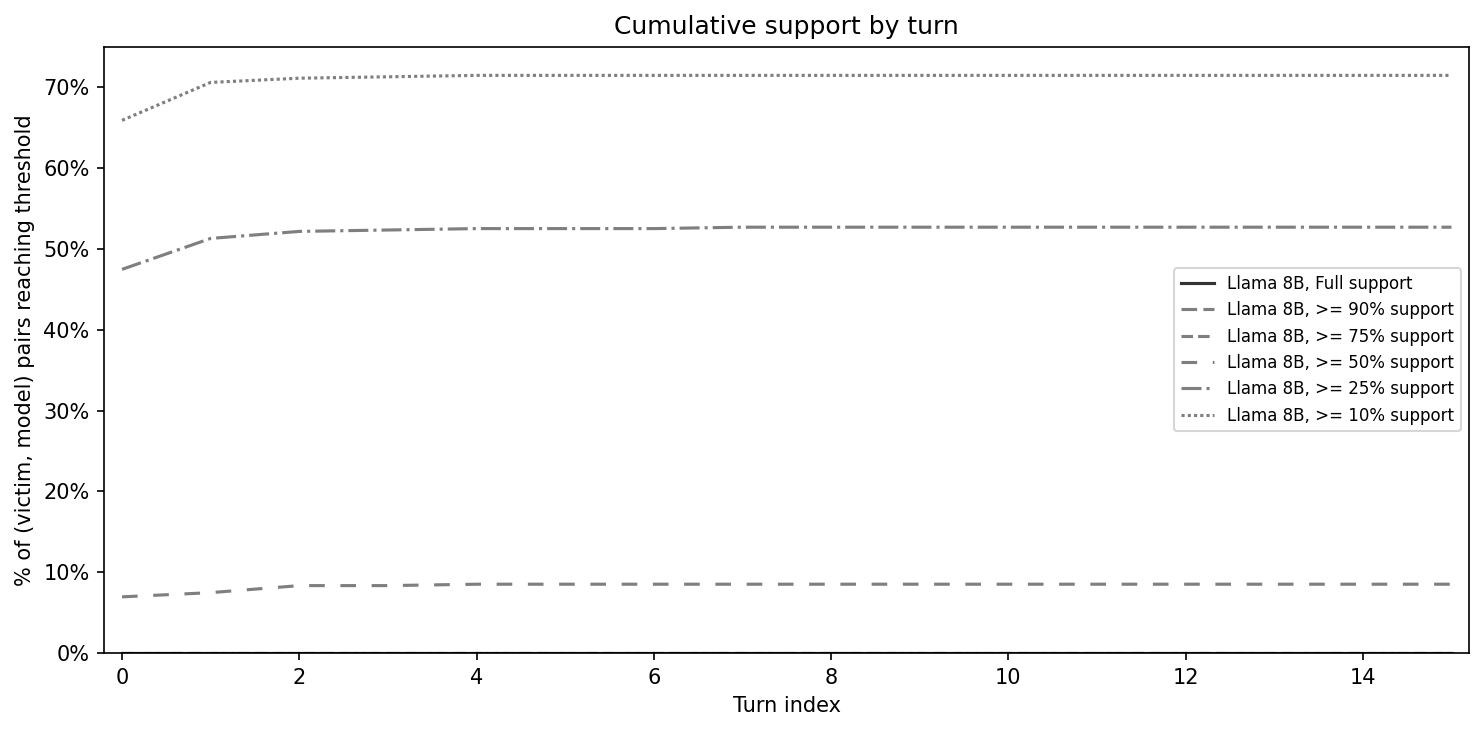
\includegraphics[width=\textwidth]{plots/evaluation/matching/all_labels_one_model/cumulative_support_curve.png}
\end{minipage}
\hfill
\begin{minipage}{0.32\textwidth}
\centering

\includegraphics[width=\textwidth]{plots/evaluation/matching/all_labels_one_model/support_ceiling_by_annotation_availability.png}
\end{minipage}
\hfill
\begin{minipage}{0.32\textwidth}
\centering
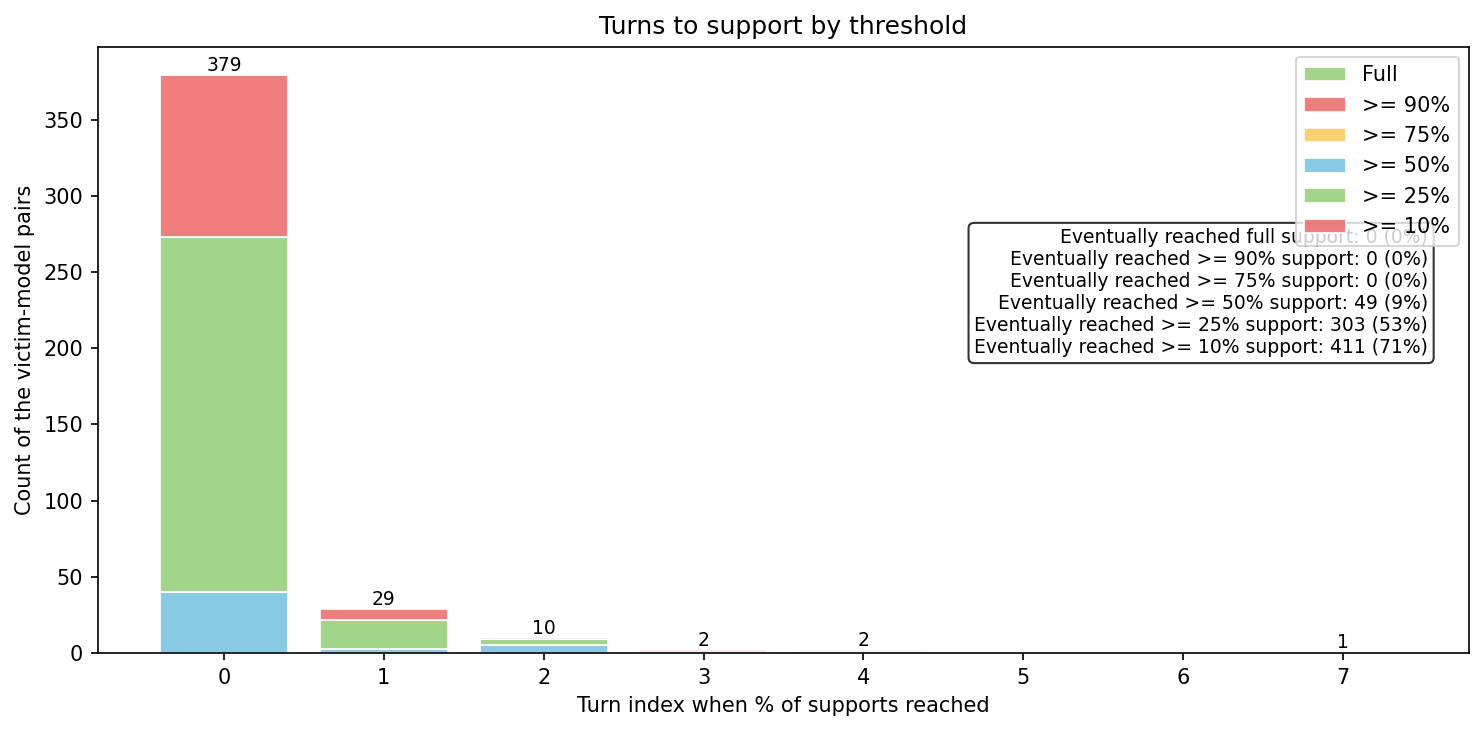
\includegraphics[width=\textwidth]{plots/evaluation/matching/all_labels_one_model/turns_to_full_support.png}
\end{minipage}
\caption{Annotation to documents mapping for all labels using a single model. Left: cumulative support curve across turns. Center: support ceiling by annotation availability. Right: number of turns to full support.}
\label{fig:matching_all_labels}
\end{figure}

The three selected labels were chosen for their low missing rates and their broad relevance, but the full codebook contains many more coded fields. Expanding the evaluation to extra categorical labels to include 15 labels in total to tests whether the pipeline can trace annotations that carry higher missing rates and that encode more specialized details. This is a harder test because full support now requires every annotated field for a victim to be grounded in the available text.

Figure~\ref{fig:matching_all_labels} reports the same three measures for the expanded label set using a single model. Full support drops to approximately 8 percent, which is expected given that every annotated label must now be matched simultaneously. At lower thresholds the pipeline still recovers evidence for a substantial share of annotations: 71 percent of pairs reach at least 10 percent support and 53 percent reach at least 25 percent. The critical constraint is visible in the support ceiling panel, where only 234 of the 453 annotated victims retain full document coverage, falling from 89 percent in the three-label setting to 52 percent when all labels are considered. The remaining 219 victims have only partial coverage because news articles that were available to the original human coders are no longer be retrievable from their sources or from the internet. This is the direct quantification of the lost documents problem introduced in the evaluation design that the pipeline can only process the documents that remain in the accessible archive, and any annotation that depended on a source that has since disappeared sets a hard ceiling on the support that can be recovered. The turn-by-turn recording that the pipeline produces makes this ceiling visible and locatable. For the annotations that can be traced, most pairs reach their threshold within the first two documents. For those that cannot be fully traced, the recording identifies precisely where the evidence trail ends, producing a concrete inventory of what the pipeline recovers and what remains beyond reach due to the state of the archive. This inventory is the practical contribution of the tracing dimension: rather than treating missing support as an unquantified limitation, the pipeline distinguishes recoverable annotations from structurally unrecoverable ones and documents the boundary between them.



\begin{table}[htbp]
    \centering
    \footnotesize
    \begin{tabular}{llp{7cm}r}
    \hline
    victim\_id & label\_key & span & offset \\
    \hline
    Veracruz\_J J R R & desenlace & ``Hasta la fecha, sigue en la b\'{u}squeda, se ha convertido en detective\dots'' & 2480 \\
    Veracruz\_J J R R & vic\_grupo\_social & ``Carmelo estudiaba arquitectura en una escuela privada de dise\~{n}o. Su c\'{i}rculo de amigos era muy grande\dots'' & 2691 \\
    N.L.\_Fabi\'{a}n H V & desenlace & ``En el expediente no hay registros del plagio ni testimonios.'' & 2585 \\
    Veracruz\_Mar\'{i}a Victoria C T & captura\_tipo & ``Seg\'{u}n Lorena, su madre y hermano fueron sustra\'{i}dos de un taxi entre la calle 13 y avenida 11, frente al DIF Municipal, el pasado 17 de abril.'' & 1254 \\
    N.L.\_Fabi\'{a}n H V & captura\_tipo & ``Los perseguidores sustrajeron al empresario del veh\'{i}culo siniestrado y se lo llevaron con rumbo desconocido en otra unidad, un Audi.'' & 4109 \\
    \hline
    \end{tabular}
    \caption{Sample extracted spans per codebook field. Each span is a verbatim excerpt from the source document; the offset records the character position where the span begins in the original text.}
    \label{tab:spans_example}
    \end{table}

\begin{table}[htbp]
    \centering
    \footnotesize
    \begin{tabular}{clllp{7.5cm}}
    \hline
    turn & doc\_id & info\_found & labels found & summary (excerpt) \\
    \hline
    0 & \_1 & FALSE & --- & (no summary produced) \\
    1 & \_2 & TRUE & desenlace, vic\_grupo\_social & ``Cuatro personas originarias de Sinaloa desaparecieron\dots\ fueron secuestrados por polic\'{i}as preventivos\dots\ y entregados a un c\'{a}rtel\dots'' \\
    2 & \_6 & FALSE & --- & (previous summary preserved unchanged) \\
    3 & \_8 & TRUE & desenlace, vic\_grupo\_social, captura\_tipo & ``\dots siete j\'{o}venes detenidos por polic\'{i}as locales y entregados a Los Zetas\dots\ la polic\'{i}a local colaboraba con el crimen organizado\dots'' \\
    \hline
    \end{tabular}
    \caption{Summary evolution across four turns for Coahuila\_Ezequiel C T. Turns~0 and~2 process noisy documents that yield no information; the pipeline preserves the previous summary unchanged. Turns~1 and~3 extract new evidence and update the running summary.}
    \label{tab:summary_turns_example}
    \end{table}

Tables~\ref{tab:spans_example} and~\ref{tab:summary_turns_example} show abbreviated examples from the full pipeline output for two of its recorded artifacts. Table~\ref{tab:spans_example} presents a sample of extracted spans. Each row records the victim identifier, the codebook field that the span addresses, the verbatim passage extracted from the source document, and the character offset where that passage begins in the original text. Table~\ref{tab:summary_turns_example} presents the turn-by-turn processing trace for a single victim across four documents. Each row records the turn index, the document identifier, whether relevant information was found in that document, which codebook labels were identified, and an excerpt of the running summary at that point. Both tables are abbreviated selections from a larger output that the pipeline produces for every victim in the corpus.

In Table~\ref{tab:summary_turns_example}, the pipeline processes four documents sequentially for one victim. At turns zero and two, the documents contain no relevant information for the victim. These are the noisy, irrelevant, or damaged pages that are common in web-scraped corpora, such as error pages, log in pages, or unrelated articles scraped alongside the target content. When the pipeline encounters such documents, it preserves the existing summary unchanged rather than letting irrelevant content dilute or degrade the evidence already collected. At turns one and three, the pipeline finds relevant information and updates the running summary accordingly. The set of supported codebook labels grows from two at turn one, where the pipeline identifies outcome and social group, to three at turn three, where it additionally identifies type of place of capture. This progressive enrichment shows that evidence for different codebook fields can be distributed across multiple documents and that the stateful design accumulates labels as informative documents are encountered. In Table~\ref{tab:spans_example}, the character offset for each extracted span records the exact position in the source document where the evidence begins. A researcher can return to the original text at the recorded offset and verify that the extracted passage appears at that location, making each piece of evidence independently checkable against the source.

The combination of verbatim spans, character offsets, and turn-by-turn processing traces means the pipeline output is auditable at the level of individual evidence claims. A researcher can follow the chain from a codebook label to the extracted passage that supports it to its character position in the source document to the specific processing turn that produced it. At the aggregate level, the support coverage analysis identifies which annotations fall within reach of the available archive and which are structurally unrecoverable because of the lost documents problem. At the instance level, the extracted spans and turn traces document precisely what was recovered and where the evidence trail ends. Together, these two dimensions produce a complete account of the annotation-to-document mapping: the pipeline does not only classify but records the evidence path for each annotation it can trace and flags the structural reason for each one it cannot.


\section{Discussion}\label{discussion}

\subsection{Ethics}\label{ethics}

Masking victim names in the dataset is an important measure to protect the privacy, dignity, and security of victims and their families. Cases involving enforced disappearance and other forms of violence often remain politically sensitive and may involve powerful actors, including criminal organizations or state agents. Publicly circulating identifiable personal information can expose victims’ relatives to intimidation, retaliation, or renewed stigmatization. By anonymizing names while preserving the relevant contextual data—such as dates, locations, and types of violations—the dataset allows researchers to analyze patterns of violence without placing individuals or families at additional risk.

Anonymization also reflects broader ethical standards in human rights research and documentation, which prioritize the protection of victims over the unrestricted dissemination of personal information. Masking identities helps prevent the re-traumatization of families and respects their right to control how their loved ones’ stories are used and shared. At the same time, the dataset remains analytically valuable because the key variables needed to study trends, language, and patterns of violence are preserved, enabling rigorous research while maintaining responsible safeguards for those directly affected by the crimes being documented.


\subsection{Error Analysis}\label{error-analysis}


Three identifiable sources of error affect the pipeline at different stages. The first is document-level noise from error pages, navigation menus, advertising banners, and topically adjacent but irrelevant content that pervade the web-scraped corpus. As established in the related work, LLM-based data standardization and error processing can handle such noise through contextual extraction and generation rather than rule-based methods. The pipeline applies this principle by using the codebook schema to focus extraction on relevant fields, so that noisy content is filtered during the extraction step itself rather than requiring a separate preprocessing stage.

The second source is missing evidence from the lost documents problem. When source articles consulted by the original coders are no longer retrievable, annotations that depended on those sources cannot be grounded regardless of extraction quality. The pipeline addresses this by recording which annotations remain unsupported after all available documents have been processed and by distinguishing structural absence of the source from the archive from extraction failure through the support ceiling and turn-by-turn recording. This makes the gap attributable and quantifiable rather than hidden within the overall accuracy figures.

The third and likely largest source of error is ambiguity in the categorization of certain texts. Some labels have options that overlap in meaning or that require contextual judgments the source text does not resolve unambiguously. When a report can reasonably support more than one category, the human coder and the model may arrive at different but defensible assignments, and this disagreement registers as a classification error even though the summary correctly preserved the relevant information. These failure modes being knowable and separable itself is a contribution to methodological transparency in computational social science, because it lets researchers make informed choices about when and how to use the output.

\subsection{Limitations}\label{limitations}

One limitation of this study is how performance is evaluated against a codebook where categories are not always sharply separable in the source text. Some reports contain descriptions that can reasonably support more than one label, so disagreement between the model output and the human annotation does not always mean that the summary failed to preserve the relevant information. In these cases, lower accuracy can partly reflect ambiguity in the source material and overlap in the taxonomy, especially for labels where valid interpretations remain close to one another. We mitigate part of this problem by merging some label options, but that adjustment also reduces category detail and makes the comparison less a direct reproduction of the original coding scheme. Even though the proposed workflow is not a full reconstruction of the original coding scheme, it is still a practical way to reconnect prior annotations to the source texts and recover traceable evidence for downstream use.

\subsection{Implications}\label{implications}

\subsubsection{Compute Time vs Human
Coding}\label{compute-time-vs-human-coding}

An important implication of the proposed workflow is that it changes the cost structure of working with inherited annotations. Recreating the earlier coding process would require retraining coders, rereading multiple reports for each victim, and reconstructing decisions that were never formally preserved, whereas the pipeline can process the same material in hours while recording each turn of evidence extraction and summary updating. The gain is therefore not only speed, but a different use of scarce expert labor. Instead of spending weeks on repetitive document cleaning, reconciliation, and aggregation, researchers can direct human effort toward validating difficult cases, resolving ambiguous categories, and interpreting substantive patterns in the data, while the repetitive parts of the task are taken care of by the LLMs. For projects that inherit valuable but imperfectly organized annotations, this makes reuse of prior coding work far more feasible than full manual reconstruction.

\subsubsection{Scalability to Other Messy
Corpora}\label{scalability-to-other-messy-corpora}

A broader value of the proposed method lies in the type of problem itaddresses rather than in the specific corpus used here. Many research projects inherit messy text and annotation collections in which reports are organized for one purpose, annotations were created for another, and the link between coded variables and supporting evidence was never formally retained. In such settings, the transferable contribution is the workflow design itself the codebook-guided extraction, evidence-linked summaries, and stateful updating across multiple documents. This portability is possible because the workflow is designed to be configurable rather than hardcoded. Separate configuration files and taxonomies can define the local labels, extraction targets, and field structure for a new corpus while leaving the underlying pipeline logic unchanged. Adapting the method to a new corpus would therefore require changing the task schema and prompts to fit the local annotation system, but not redesigning the full logic of the pipeline. This suggests that the approach can generalize to other legacy corpora where researchers need to recover usable and traceable structured text from noisy materials without repeating the original annotation process from the beginning.

\subsubsection{Downstream Tasks}\label{downstream-tasks}

When developing new research projects using the UMN dataset, we are particularly interested in analyzing how violence is portrayed, described, or obscured through language in public reporting, especially in ways that prevent the systematic identification of human rights and international crimes. Our work focuses on identifying the use of euphemisms, ambiguous terminology, and narrative framing that mask patterns of violence and make it more difficult to establish the widespread or systematic nature of abuses—an essential requirement for proving international crimes before courts. By analyzing large corpora of media reports and related documentation, we aim to understand how linguistic practices can shape the visibility of violence and influence whether certain acts are recognized as human rights violations.

One specific focus of our research using the UMN dataset concerns the terminology that emerged during Mexico’s so-called “War on Drugs,” declared by President Felipe Calderón in 2006. During this period, journalists increasingly used the term “levantón” (“big lift”) to describe events involving the deprivation of liberty followed by the disappearance of individuals whose fate and whereabouts remained unknown. Although some journalists now employ more accurate terminology, many reports still frame disappearances primarily as ordinary criminal acts rather than as serious human rights violations, often overlooking the possible role of the state through action, tolerance, or omission. Our research seeks to examine how such language contributes to the normalization or depoliticization of enforced disappearance in public discourse.

Presenting disappearances as isolated crimes creates several analytical and legal problems. First, it reduces the event to a single act of deprivation of liberty rather than recognizing enforced disappearance as a continuous and ongoing crime that persists as long as the person’s fate remains unknown. Second, it obscures the multiple human rights violations involved, including violations of the rights to life, personal integrity, and juridical personality, and ignores the broader circle of victims affected by the disappearance. Finally, it conceals the possible involvement of the state, which is central to the legal definition of enforced disappearance. The use of terms like “levantón” is particularly problematic because it originates in the lexicon of organized crime and functions as a euphemism that masks what may in fact be enforced disappearance. Through systematic analysis of this language, our research seeks to reveal how linguistic framing can obscure patterns of violence that are essential for legal accountability and human rights documentation.


\section{Conclusion and Future Work}\label{conclusion-and-future-work}

The central obstacle in working with inherited messy text is not noise alone, but the broken connection between prior human coding and the source evidence on which that coding depended. The proposed codebook-guided extractive summarization workflow addresses that gap by producing clean, evidence-linked summaries that remain traceable to the original reports and usable for downstream language model tasks. It offers a practical way to preserve and reactivate costly human judgment that would otherwise remain trapped inside legacy annotations, while shifting scarce expert labor away from repetitive reconstruction and toward validation, interpretation, and substantive analysis.

Future work can build on this recovered representation as research infrastructure for organizing text datasets by a schema driven by codebook definitions for cumulative human rights research, future investigations, historical reconstruction, and accountability over time. In that role, it can help sustain shared evidence across long term collaborative projects and make structured documentation more usable for local organizations, independent researchers, victims, and affected communities.

\section*{References}

\appendix
\section{Appendix}\label{appendix}

\newpage
\printbibliography

\end{document}
